% Usar papel de carta y fuente de 11 putos.
\documentclass[12pt,paper=a4, spanish]{report}
% Ajustar los margenes de la hoja (el izquierdo es mayor que el derecho para el encuadernado).
\usepackage[tmargin=1in, rmargin=0.8in, bmargin=1in, lmargin=0.8in]{geometry}

% Utilización de las codificaciones, latin1 y utf8 para windows y gnu/linux respectivamente.
\usepackage[latin1,utf8]{inputenc}
\usepackage{times}
\usepackage[T1]{fontenc} 
\usepackage[scaled]{uarial}
%\usefont{T1}{arial}{m}{n}

%\usepackage{ucs}

% Utilizar el idioma español para la división de palabras en sílabas al final del renglón.
\usepackage[spanish,activeacute]{babel}

% El paquete graphicx maneja los graficos que se generan en el documento.
\usepackage{graphicx}
\usepackage{color}

% El paquete acronym brinda la posibilidad de utilizar los acronimos de forma sencilla.
\usepackage{acronym}

% El paquete fancyhdr es usado para las cabeceras de página (headers).
\usepackage{fancyhdr}
\usepackage{fancybox}
\setlength{\headheight}{15pt}
\renewcommand{\footrulewidth}{0.4pt}



% El paquete hyperref es usado para manejar lon vinculos a referencias en el documento dijital.
\usepackage{hyperref}

% Configurar el paquete hyperref para que pinte de color negro todos los vinculos.
\hypersetup{colorlinks=true,
	linkcolor=black,
	citecolor=blue,
	filecolor=black,
	urlcolor=blue,
	pdfauthor=  Luis Andr�s Valido Fajardo
}

% Usar interlineado de 1.5
\renewcommand{\baselinestretch}{1.5}

%Paquete para poner la primera línea de un párrafo más grande que las demás
\usepackage{lettrine}
\renewcommand{\LettrineFontHook}{\fontfamily{ppl}}%


% Fuente clon de Arial
% \renewcommand{\rmdefault}{phv}
% \renewcommand{\sfdefault}{phv}

%Para símbolos matemáticos
\usepackage{amsmath}

%Para poder escribir códigos de otro lenguajes sin problemas
\usepackage{verbatim}

%Paquete para hacer comentarios
\usepackage[colorinlistoftodos]{todonotes}

%Paquetes para la marca de agua
\usepackage{draftcopy}
\usepackage{type1cm}
\usepackage{eso-pic}
\usepackage{everypage}


%Incluye la bibliografía en el índice
\usepackage[nottoc]{tocbibind}

%enumerar las figuras a partir del capitulo
\usepackage{chngcntr}
\counterwithin{figure}{chapter}
\counterwithin{table}{chapter}

% para formatear la presentaci�n de los capitulos
\usepackage{titlesec}  
 

%Paquetes para trabajo con tablas
\usepackage{longtable}
\usepackage{colortbl}
\definecolor{Light}{gray}{.80}
\definecolor{Dark}{gray}{.20}


%Aquí se definen las extensiones de las imagenes que se van a usar
\DeclareGraphicsExtensions{.jpg, .bmp, .png}




\usepackage[backend=bibtex,
style=authoryear,citestyle=authoryear-comp,natbib=true,
sorting=nyvt,
doi=true,
isbn=true,
url=true,
firstinits=true,
dashed=false,
hyperref=true]{biblatex}


\DeclareCiteCommand{\cite}
{\usebibmacro{prenote}}
{\usebibmacro{citeindex}%
	\printtext[bibhyperref]{\usebibmacro{cite}}}
{\multicitedelim}
{\usebibmacro{postnote}}

\DeclareCiteCommand*{\cite}
{\usebibmacro{prenote}}
{\usebibmacro{citeindex}%
	\printtext[bibhyperref]{\usebibmacro{citeyear}}}
{\multicitedelim}
{\usebibmacro{postnote}}

\DeclareCiteCommand{\parencite}[\mkbibparens]
{\usebibmacro{prenote}}
{\usebibmacro{citeindex}%
	\printtext[bibhyperref]{\usebibmacro{cite}}}
{\multicitedelim}
{\usebibmacro{postnote}}

\DeclareCiteCommand*{\parencite}[\mkbibparens]
{\usebibmacro{prenote}}
{\usebibmacro{citeindex}%
	\printtext[bibhyperref]{\usebibmacro{citeyear}}}
{\multicitedelim}
{\usebibmacro{postnote}}

\DeclareCiteCommand{\footcite}[\mkbibfootnote]
{\usebibmacro{prenote}}
{\usebibmacro{citeindex}%
	\printtext[bibhyperref]{ \usebibmacro{cite}}}
{\multicitedelim}
{\usebibmacro{postnote}}

\DeclareCiteCommand{\footcitetext}[\mkbibfootnotetext]
{\usebibmacro{prenote}}
{\usebibmacro{citeindex}%
	\printtext[bibhyperref]{\usebibmacro{cite}}}
{\multicitedelim}
{\usebibmacro{postnote}}

\DeclareCiteCommand{\textcite}
{\boolfalse{cbx:parens}}
{\usebibmacro{citeindex}%
	\printtext[bibhyperref]{\usebibmacro{textcite}}}
{\ifbool{cbx:parens}
	{\bibcloseparen\global\boolfalse{cbx:parens}}
	{}%
	\multicitedelim}
{\usebibmacro{textcite:postnote}}


%CONFIGURACIONES PARA LA MARCA DE AGUA	
\newenvironment{water}{\AddEverypageHook{\waterb}}{\AddThispageHook{\waterb}\AddEverypageHook{\watere}}

\makeatletter
\newcommand{\waterb}{
\AddToShipoutPicture*{%
            \setlength{\@tempdimb}{.5\paperwidth}%
            \setlength{\@tempdimc}{.5\paperheight}%
            \setlength{\unitlength}{1pt}%
            \put(\strip@pt\@tempdimb,\strip@pt\@tempdimc){%
        \makebox(0,0){\rotatebox{45}{\textcolor[gray]{0.97}%
        {\fontsize{6cm}{6cm}\selectfont{}}}}%
            }%
}}
\makeatother

\makeatletter
\newcommand{\watere}{
\AddToShipoutPicture*{%
            \setlength{\@tempdimb}{.5\paperwidth}%
            \setlength{\@tempdimc}{.5\paperheight}%
            \setlength{\unitlength}{1pt}%
            \put(\strip@pt\@tempdimb,\strip@pt\@tempdimc){%
        \makebox(0,0){\rotatebox{45}{\textcolor[gray!10]{1}%
        {\fontsize{6cm}{6cm}\selectfont{DRAFT}}}}%
            }%
}}
\makeatother

% Incluir el fichero donde se definen o redefinen algunos comandos


\definecolor{tcA}{rgb}{0.9,0.9,0.9}

\newcommand\BackgroundPic{
	\put(0,0){
		\parbox[b][\paperheight]{\paperwidth}{%
			\vfill
			\centering
			
\includegraphics[width=\paperwidth,height=\paperheight,
			keepaspectratio]{./img/logo6.png}%
			\vfill
}}}

\newcommand{\universidad}{\large{Universidad de Matanzas }}
\newcommand{\facultad}{\large{Facultad de Ciencias Sociales y Humanidades}}

\newcommand{\espacios}{\vspace{0.5in}}

\newcommand{\espaciosH}{\hspace{0.5in}}

\newcommand{\entidad}
{
 	\begin{tabular}{c}
 		
 		\universidad \\
 		\facultad \\ 
 		\espacios \\
 		
 	\end{tabular}
}

\newcommand{\logoUniversidad}{
\includegraphics[scale=0.69]{img/logo_umcc.png}}
\newcommand{\logoFacultad}{
\includegraphics[scale=0.03]{img/logo_facultad_fcsh_negro.png}}

\newcommand{\banner}
{
 \espacios
\begin{center}
\begin{tabular}{ccc}

\logoUniversidad  & \espaciosH \entidad  & \espaciosH \logoFacultad  \\

\end{tabular}
\end{center}


 \espacios
 }


% Escribir el titulo de la tesis que va a exponer.
\newcommand{\tituloTesis}{ INFORME DE AUTOEVALUACIÓN
\\ CARRERA: GESTIÓN SOCIOCULTURAL PARA EL DESARROLLO}

\newcommand{\tituloTesisPrimeraPagina}{ {\fontsize{17pt}{17pt}\selectfont \tituloTesis} }


% Cambiar el tipo de trabajo si es necesario.
\newcommand{\nombreTipoTesis}{ {\fontsize{14pt}{14pt}\selectfont Trabajo de Diploma  para la Obtención del Título de Ingeniero Informático}}

% Cambiar los nombres de los autores.
\newcommand{\autorUNO}[1]{{\fontsize{16pt}{16pt}\selectfont #1}}
\newcommand{\autorFIRMA}[1]{{ #1}}

\newcommand{\programmer}{Randy Mederos Santana}
\newcommand{\taskdevelop}{Desarrollo}
\newcommand{\taskdesign}{Diseño}
% Cambiar el nombre del tutor y co-tutor.
\newcommand{\tutorUNO}[1]{{\fontsize{16pt}{16pt}\selectfont #1}}
%\newcommand{\coTutor}{}

% Cambiar el cargo del tutor y co-tutor
%\newcommand{\cargoTutor}{Cargo del tutor}
%\newcommand{\cargoCoTutor}{Cargo del co-tutor}

% Cambiar la fecha de confección de la tesis. Por defecto es el día de hoy
\usepackage{datetime}


\renewcommand{\today}{\number \year} 
\newcommand{\fecha}{\large{\today}}





\newcommand{\titulo}{\tituloTesisPrimeraPagina\espacios}

\newcommand{\tipoTesis}{\nombreTipoTesis \espacios \espacios}

\newcommand{\autores}
{
	
    \begin{center}
    \begin{tabular}{rl}
    {\fontsize{16}{16} \selectfont  Autor:}  & \autorUNO{Randy Mederos Santana}  \vspace{1.5em}   \\
                       
    {\fontsize{16}{16} \selectfont Tutor:}    & \tutorUNO{M.Sc. Luis Andrés Valido Fajardo}    \\
    %\large{\bf Co-Tutor:} & \large{\coTutor}
    \end{tabular}
    \end{center}
    \vspace{1.0in}
}

\newcommand{\ciudadFecha}{{\fontsize{14pt}{14pt} \selectfont Matanzas, 2022}}

\newcommand{\fillDia}{\makebox[0.3in]{\hrulefill}\space}
\newcommand{\fillMes}{\makebox[1in]{\hrulefill}\space}
\newcommand{\fillAnno}{\makebox[0.5in]{\hrulefill}}

\newcommand{\firma}{\makebox[2in]{\hrulefill}}

\newcommand{\firmaTesis}
{
    \begin{center}
    \begin{tabular}{ccc}
             &  \firma  &     \\
             &  \autorFIRMA{Randy Mederos Santana} &   \\
    \end{tabular}
    \end{center}
}

\newcommand{\comentario}[2][]
{
	\todo[caption={#2}, size=\small, #1, inline,color={red!100!green!8},bordercolor=red,linecolor=red]
	{
	  \renewcommand{\baselinestretch}{1.2}\selectfont#2\par
	}
}

%Biliografia
%\RequirePackage[round, authoryear]{natbib}
%\usepackage[numbers]{natbib}
%\usepackage[sort,round,colon,authoryear]{natbib}
%\usepackage{lipsum}

\renewcommand{\chaptertitlename}{\uppercase{Variable}}
\renewcommand{\tablename}{Tabla}
\newcommand{\mc}[3]{\multicolumn{#1}{#2}{#3}}
% Formateo de la presentacion del titulo de cada capítulo
\titleformat{\chapter}[hang] 
{\fontsize{14pt}{14pt}\bfseries}{\chaptertitlename\ \thechapter:}{0.1em}{}
\titlespacing*{\chapter}{0pt}{0pt}{15pt} 
\titlespacing*{\section}{0pt}{5pt}{5pt} 

%Quitar el margen a la primera línea de los párrafos
\setlength{\parindent}{0in}

%Formato de las secciones




\titleformat{\section}{\normalfont\fontsize{12pt}{12pt}\bfseries}{\thesection}{1em}{}
\titleformat{\subsection}{\normalfont\fontsize{12pt}{12pt}\bfseries}{\thesubsection}{1em}{}
\titleformat{\subsubsection}{\normalfont\fontsize{12pt}{12pt}\bfseries}{\thesubsubsection}{1em}{}

\setcounter{secnumdepth}{3}
\setcounter{tocdepth}{2}

\renewcommand{\tablename}{Tabla}
\def\tablename{Tabla}

\begin{document}

\begin{titlepage}
    \begin{center}

%   Logo de la universidad
    \banner

    %\vspace*{\fill}
%   Titulo de la tesis:
    \titulo

%   Tipo de tesis:
    \begin{figure}[h!]
    	\centering
    	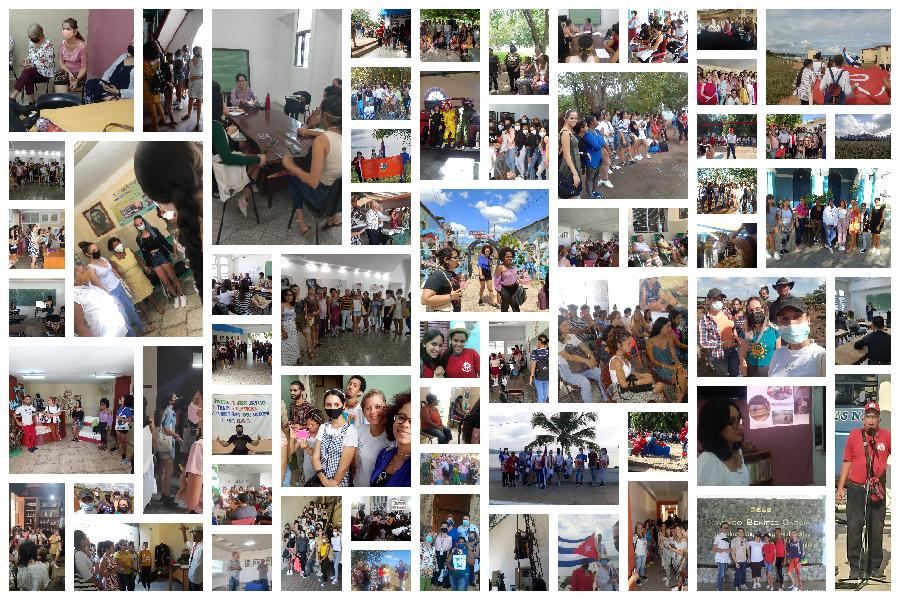
\includegraphics[width=1.0\linewidth]{img/banner}
    	\label{fig:banner}
    \end{figure}
    

    \vspace*{\fill}
%   Lugar y fecha de confección de la tesis
    \ciudadFecha

    \end{center}
\end{titlepage}


		%Para renombrar los nombres de table y figure por tabla y figura respectivamente.
  


    
    
  
    \AddToShipoutPicture{\BackgroundPic}
    \tableofcontents % Índice general
    \pagebreak
    
   \pagestyle{fancy}
   \fancyhead[LO,CE]{
\includegraphics[scale=0.27]{img/logo_umcc2.png} 
   	\begin{minipage}{0.5\textwidth} % 60% de la p�g
   		\begin{flushleft}
   			\vspace*{-0.4in}
   			\centering Departamento de Estudios Socioculturales\\
   			\centering Carrera de Gesti\'on Sociocultural para el Desarrollo
   	\end{flushleft}
   \end{minipage}
}
   \fancyhead[RO,CE]{
\includegraphics[scale=0.013]{img/logo_facultad_fcsh.png}
   		\begin{minipage}{0.3\textwidth} % 60% de la p�g
   			\begin{flushright}
   				\vspace*{-0.4in}
   				\centering Autopista a Varadero 3 $\frac{1}{2}$ Km \\
   				\centering Matanzas, Cuba
   		\end{flushright}\end{minipage}
	}
   \fancyfoot[LO,CE]{}
   \fancyfoot[RO,CE]{}
   \fancypagestyle{plain}{\pagestyle{fancy}}
   
   
   \addcontentsline{toc}{chapter}{\fontsize{14pt}{14pt} CARACTERIZACI\'ON DE LA CARRERA GESTI\'ON SOCIOCULTURAL PARA EL DESARROLLO} 
   \chapter*{CARACTERIZACI\'ON DE LA CARRERA GESTI\'ON SOCIOCULTURAL PARA EL DESARROLL}
   \input{tex_files/caracterizacion}
    \pagebreak
   
   
  
   
    
   \chapter{PERTINENCIA E IMPACTO SOCIAL}
   \section{Proyección de la profesión hacia el territorio y/o el país}
%\addcontentsline{toc}{section}{\large Proyección de la profesión hacia el territorio y/o el país }

El Departamento de Estudios Socioculturales, donde radica la carrera Gestión Sociocultural para el Desarrollo, durante los últimos cinco años ha logrado afianzar los vínculos de los profesores y estudiantes con la solución de los problemas del territorio y/o del país. De esta manera se cumple con el principal encargo de la carrera, que es formar profesionales centrados en los procesos de gestión sociocultural dirigidos a potenciar el desarrollo humano, individual y colectivo, que incide directamente en el enriquecimiento espiritual, fortalecimiento de la identidad cultural y nacional, en la calidad de la vida colectiva y la capacidad de participación de la población en el desarrollo social, en correspondencia con los Lineamientos de la Política Económica y Social del Partido y la Revolución, el Plan Nacional de Desarrollo Económico y Social 2030 y los 17 objetivos para el desarrollo sostenible declarados en la Agenda 2030. 

En la provincia de Matanzas la carrera está abierta en la Universidad de Matanzas (sede central) y en siete de sus municipios: Cárdenas, Colón, Jovellanos, Jagüey Grande, Calimete, Limonar y Los Arabos. La labor que realiza desde cada una de sus sedes, hace que posea una elevada pertinencia, avalada por la contribución al estudio, tratamiento y solución a problemas del territorio, con la participación de los estudiantes y profesores del claustro.

El trabajo con el banco de problemas del territorio se organiza desde el colectivo de carrera, colectivo de la Disciplina Principal Integradora y los colectivos de año, con el protagonismo de la FEU en las Sociedades Científicas Estudiantiles (SCE), en correspondencia con el objetivo integrador de cada año académico y con las líneas de investigación. A partir de estas, teniendo en cuenta el trabajo interdisciplinar, los modos y esferas de actuación profesionales, las exigencias del modelo del profesional y la ejecución del componente laboral investigativo se realizan las orientaciones de la actividad científica de profesores y estudiantes.

Constituye un elemento fundamental en la carrera la formación de cuatro SCE en líneas de investigación, que trabajan las siguientes temáticas: desarrollo local e intervención comunitaria, procesos culturales cubanos, extensión universitaria y gestión integral del patrimonio. A estas temáticas se asocian los estudiantes de la carrera quienes unidos a sus profesores / tutores desarrollan acciones desde la docencia, la investigación y la extensión.

A partir de lo expuesto, se realizan trabajos de curso e investigaciones que aportan resultados científicos que tributan a proyectos de investigación y generalmente se concretan en trabajos de diploma. Materializadas en propuestas de soluciones totales o parciales a problemáticas relacionadas a la gestión sociocultural, donde los estudiantes ponen en práctica sus modos y esferas de actuación profesionales para la prevención de salud, medioambiental, de género, social, la gestión turística, la gestión cultural de instituciones, gestión sociocultural del patrimonio, de la información y el conocimiento, entre otras.

Hasta la fecha se han presentado 3 convocatorias a ejercicios de culminación de estudios del Plan de Estudio E, en la carrera Gestión Sociocultural para el Desarrollo, para un total de 36 graduados. De ellos, en el curso 2019-2020 y curso 2021, fueron eximidos estudiantes por resolución rectoral en período de Covid 19 y hubo presentados en examen estatal, por lo que, de un total de 27 egresados en estos cursos, 13 (48.1\% con respecto a la cantidad de egresados), presentaron Trabajos de Diploma que aportan resultados científicos en sistemas de actividades y planes de acciones para implementarse en instituciones educativas, instituciones culturales, comunidades, medios de comunicación (la radio), en el sector no estatal y en el sector del turismo, en los siguientes temas:

\begin{itemize}
	\setlength\itemsep{-0.5em}
	\item El proceso de gentrificación en el poblado de Boca de Camarioca del municipio Cárdenas. 
	\item Gestión medioambiental en los niños con discapacidad intelectual del 2do ciclo de la Institución Educativa \emph{Franklin Gómez}.
	\item Gestión turística del patrimonio cultural y participación comunitaria en el Consejo Popular René Fraga Moreno de Colón.
	\item La participación de los niños con discapacidad intelectual de segundo ciclo de la Institución Educativa Franklin Gómez que contribuya a la integración con la comunidad.
	\item Gestión turística en el proceso de rehabilitación de la Zona Priorizada para la Conservación del Centro Histórico Urbano de la ciudad de Matanzas.
	\item Inserción social de pacientes rehabilitados. Estudio de caso: Área de Neurodesarrollo.
	\item La emisora Radio Victoria de Girón como vía de formación cultural para los adolescentes jagüeyenses.
	\item Política Cultural Cubana en el sector no estatal: caso de estudio CNA Decorarte
	La promoción del Taller de Creación Literaria Pablo Neruda de la Universidad de Matanzas (2018-2021)  
	\item Prevención de la violencia intrafamiliar en la Comunidad de Santa Ana, municipio Limonar, provincia Matanzas 
	\item La gestión interpretativa del patrimonio urbano matancero para el desarrollo del turismo cultural
	\item Los estudios de violencia de género desde la extensión universitaria en la Universidad de Matanzas
	\item Propuesta de recorrido interpretativo en el Museo Juan Gualberto Gómez de Unión de Reyes. 
\end{itemize}

En el curso 2022, de un total de 9 estudiantes evaluados, (66.7\% con respecto a la cantidad de egresados), presentan trabajos de diploma, con los temas siguientes:  

\begin{itemize}
	\setlength\itemsep{-0.5em}
	\item Turismo literario en las editoriales matanceras mediante la interpretación del patrimonio.
	\item Las TIC en la socialización del patrimonio en el Centro Histórico Urbano de Matanzas.
	\item Los Círculos de interés: una vía para la educación patrimonial en las escuelas primarias.
	\item La educación patrimonial para el desarrollo sociocultural desde el museo \emph{Constantino Barredo Guerra} de Perico.
	\item Gestión de la comunicación en las actividades de extensión universitaria.
	\item Participación comunitaria de las personas que viven con discapacidad físico motoras en las actividades culturales.
\end{itemize}

Como se ha planteado, la participación y/o coordinación de proyectos por parte de profesores del claustro posibilita la inserción de estudiantes e investigadores, asume la fortaleza multidisciplinaria de los mismos y por ello contribuye y beneficia el trabajo interdisciplinar. En dichos proyectos se han ejecutado investigaciones que tributan a resultados científicos presentados en eventos internacionales (UNISOC - Universidad Sociedad), en talleres, Jornadas Científicas Estudiantiles, en ejercicios de culminaciones de estudio, etc. Proponen también la formación posdoctoral, doctorales y de maestría. Estos proyectos son:  

\begin{itemize}
	\setlength\itemsep{-0.5em}
	\item Proyecto Estudios socioculturales para el desarrollo sostenible: UM-DECORARTE (PNAP). Dr. C. Rosa Elvira Alfonso Ramos. (se propone la evaluación del impacto sociocultural de la Cooperativa No Agropecuaria DECORARTE, en la comunidad intra y extra universitaria).
	\item Gestión sociocultural para el desarrollo local en el Consejo Popular Matanzas Este (PAPT). Dr. C. Ana Gloria Peñate Villasante. (atiende un problema de investigación relacionado con el apoyo al diseño y manejo de destinos turísticos sostenibles. Se plantea como objetivo general contribuir al desarrollo del turismo cultural a partir de la gestión turística del patrimonio en el Consejo Popular Matanzas Este, específicamente en la zona declarada Monumento Nacional (MN).
	\item VIDAS en el Rabí (PAPT). Dr. C. Odalis Alberto Santana. (responde a una problemática demandada por AZCUBA, ante la necesidad de reanimar el desarrollo sociocultural en la comunidad Jesús Rabí, donde se encuentra uno de los polos productivos más importantes del país, corre el riesgo de la pérdida de fuerza laboral, entre otras causas, por la emigración de sus habitantes hacia otros territorios. Tiene como objetivo general contribuir al desarrollo sociocultural de la comunidad Jesús Rabí en el municipio de Calimete; a partir de la articulación del trabajo comunitario y la gestión sociocultural en este sitio).
	
\end{itemize}

Se cuenta con otros proyectos de investigación, donde participan profesores y estudiantes del claustro, estos son:

\begin{itemize}
	\setlength\itemsep{-0.5em}
	\item Proyecto Identidad y realidad cubana: estudio sociocultural del impacto de las transformaciones socioeconómicas en el centro de Cuba (PAP) (I+D+I). M. Sc. Soilen Cedeño Solís. (Con el propósito de fundamentar desde la perspectiva sociocultural el impacto de las transformaciones socioeconómicas en la identidad cultural en el centro de Cuba).
	\item La Competencia Comunicativa Intercultural en el Discurso de Interpretación Patrimonial para el Desarrollo Local del Turismo de Ciudad. (PNAP, 2022-2024). Dr. C. Jorge Luis Rodríguez Morell. (Con el objetivo de contribuir a la construcción progresiva de la competencia comunicativa intercultural en el discurso de interpretación patrimonial de los actores comunicativos fundamentales asociados al desarrollo local del turismo de ciudad).
	\item Patrimonio cultural y formación: patrimonio cultural universitario (PCU), historia, educación patrimonial y desarrollo local (PNAP, 2022-2024). Dr. C. Lissette Jiménez Sánchez. (Se propone como resultado principal un programa educativo, que valoriza el PCU y significa su contribución a la formación integral y diversificada de profesionales en la Universidad de Matanzas).
	\item Perfeccionamiento de la Gestión Universitaria (PNAP). Dr. C. Lourdes Tarifa Lozano. (Con el objetivo de perfeccionar el sistema de gestión universitaria orientado a la calidad que facilite el funcionamiento adecuado de la institución de educación superior, teniendo en cuenta tanto el marco legal como la responsabilidad social establecida y vinculado al trabajo inherente del sistema de dirección).
\end{itemize}

En el caso de los proyectos socioculturales A Moverse por el Cambio, en el de la Galería Joel Peláez y AfroAtenas, aportaron resultados para eventos, Jornadas Científicas Estudiantiles y trabajos de diploma en los cursos 2017-2018, 2018-2019 y 2019-2020.

Se aprecia un gradual incremento en la superación y formación de los docentes del Departamento de Estudios Socioculturales. Como resultado de este proceso continuo, 3 profesoras se encuentran cursando maestrías que tributan a: Administración de Empresas, Didáctica de las Humanidades y en Estudios Sociales y Comunitarios; en formación doctoral se encuentran 5 profesores: 3 en Ciencias de la Educación, 1 en Ciencias Históricas y 1 en Ciencias Económicas. Esta superación continua incrementa el impacto de la carrera hacia el territorio matancero.

Existe una estrecha colaboración con las entidades del territorio, entre ellas: la Dirección Provincial de Cultura, el Centro de Superación para la Cultura, la Delegación Territorial de Ciencia Tecnología y Medio Ambiente (CITMA), Museo de Arte Matanzas, Ediciones Vigía, Asociación Hermanos Saiz, Dirección Provincial de Salud, Dirección Provincial de Trabajo y Seguridad Social, la Federación de Mujeres Cubanas, entre otras.

Estas relaciones institucionales han posibilitado se evidencie el impacto social de la carrera en la provincia, ya que ha diversificado la mirada en torno a la formación que recibe el egresado de la carrera Gestión Sociocultural para el Desarrollo.

El Taller Cultura - Universidad es un ejemplo de los vínculos entre organismos empleadores, la carrera y los egresados de la misma. Este evento, que cuenta con más de quince ediciones, se ha convertido en un espacio de integración entre la primera unidad docente de la carrera, el Departamento de Investigación y Desarrollo de la Dirección Provincial de Cultura (UDI) y otros Organismos de la Administración Central del Estado (OACE).

Se desarrollan actividades en proyectos de investigación, maestrías, diplomados, especialidades y doctorados vinculados a diferentes instituciones sociales y educacionales, tales como: el Departamento de Estudios de Ciencias de la Educación de la Universidad de Matanzas (DEDES), Facultad de Ciencias Pedagógicas, Facultad de Ciencias Técnicas, el CEAT, y Departamento de Historia y Marxismo - Leninismo, entre otras.

De igual modo se fortalece el impacto social en las instituciones y la formación posgraduada, con los posgrados impartidos por el Departamento de Estudios Socioculturales en el período evaluado:\\

\underline{\textbf{Año 2018:}}

\begin{itemize}
	\setlength\itemsep{-0.5em}
	\item Posgrado: Gestión y Desarrollo cultural en el ámbito de los museos. Profesora: Dr. C. Ana Gloria Peñate Villasante.
	\item Posgrado: Gestión de marketing en la comercialización de la cultura. Profesor: M. Sc. Andrés Rodríguez Reyes.
\end{itemize}

\underline{\textbf{Año 2019:}}

\begin{itemize}
	\setlength\itemsep{-0.5em}
	\item Posgrado: ¿Cómo escribir un documento científico? Profesora: Dr. C. Rosa Elvira Alfonso Ramos.
	\item Posgrado: Las religiones populares cubanas de origen africanas en Matanzas. M. Sc. Profesor: Andrés Rodríguez Reyes. 
\end{itemize}

\underline{\textbf{Año 2020:}}

\begin{itemize}
	\setlength\itemsep{-0.5em}
	\item Posgrado: Principios Fundamentales de la museología. Profesora: Dr. C. Ana Gloria Peñate Villasante.
	\item Posgrado: Las religiones populares cubanas de origen africanas en Matanzas. Profesor: M. Sc. Andrés Rodríguez Reyes.
	\item Posgrado: Gestión de marketing en la comercialización de la cultura. Profesor: M. Sc. Andrés Rodríguez Reyes. 
\end{itemize}

\underline{\textbf{Año 2021:}}

\begin{itemize}
	\setlength\itemsep{-0.5em}
	\item Posgrado: Gestión integral del Patrimonio cultural. Profesora: Dr. C. Ana Gloria Peñate Villasante.
	\item Posgrado: Gestión de marketing en la comercialización de la cultura. Profesor: M. Sc. Andrés Rodríguez Reyes.
\end{itemize}

\underline{\textbf{Año 2022:}}

\begin{itemize}
	\setlength\itemsep{-0.5em}
	\item Posgrado: Teoría y Práctica de la Interpretación del Patrimonio Profesores: Dr. C. Ana Gloria Peñate Villasante y Lic. Guillermo Alfredo Jiménez Pérez.
	\item Posgrado: Diseño Teórico - Metodológico de la Investigación Social Profesora: Dr. C. Ana Gloria Peñate Villasante.
	\item I Edición del Diplomado en Gestión Sociocultural para el Desarrollo Local y Humano. Claustro de Profesores del Departamento de Estudios Socioculturales.
\end{itemize}

Se comenzó en el curso 2022 el Programa de Técnico Superior de Ciclo Corto en Trabajo Social, siendo su matrícula los trabajadores sociales del municipio de Matanzas, en estrecho vínculo y dando respuesta a las necesidades de la Dirección Provincial de Trabajo y Seguridad Social en el territorio. 
 
La carrera cuenta en su claustro con profesionales expertos en organismos nacionales, en tribunales de cambio de categoría docente y mínimo de doctorado, miembros del Consejo Científico de la Universidad y miembros de la Junta de Acreditación Nacional (JAN), Coordinador Nacional del programa de posgrado en la Red de Educación Superior, miembro del comité nacional de expertos de Tecnología Educativa del MES, miembros de la COPED y miembros de la Comisión de Grado Científico de la UM. 

Los egresados de la carrera que imparten docencia pueden optar por la Maestría Didáctica de las Humanidades y la Maestría en Estudios Sociales y Comunitario, en la que parte de su Comité Académico y profesores son docentes del claustro de la carrera. También se mantiene la convocatoria del Diplomado en Gestión Sociocultural para el Desarrollo Local y Humano.

Los profesores y estudiantes han participado en tareas de impacto, entre ellas: acciones recuperativas de eventos meteorológicos, en la gestión de las muestras y exposiciones que se presentan en la Galería Joel Peláez, ubicada en el Departamento de Estudios Socioculturales. Han contribuido a diagnósticos con la aplicación de encuestas a la población, como fue el caso de INNOVAMATANZAS en el curso 2018, en el curso 2019-2020 se encuestaron a jóvenes matanceros para un estudio nacional sobre adolescencias y juventudes, coordinado por la UJC. Ya en el curso 2022 se promueve a nivel nacional el Movimiento Sembrar Con Ciencia, donde participaron los estudiantes de 4to año en las actividades realizadas en la provincia de Matanzas. 

En el periodo de la COVID-19 los profesores y estudiantes estuvieron incorporados a las pesquisas, a la zona roja, al trabajo en organopónico y a otras actividades convocadas para el enfrentamiento a la pandemia.

El trabajo comunitario es otro de los aspectos de interés en las tareas de impacto social, por lo que profesores y estudiantes del claustro han estado presentes en el apoyo a las comunidades en programas del municipio de Matanzas de transformación social. Específicamente en la comunidad 43 del Consejo Popular Playa y en el Consejo Popular Peñas Altas. 

Se ha continuado contribuyendo al programa de la universalización de la enseñanza en la provincia, tanto en las actividades metodológicas, capacitaciones, entrenamiento para la preparación científica y metodológica de los profesores en las asignaturas correspondientes.
Profesores del claustro pertenecen al Proyecto Antenas que comienza a finales del 2022, Proyecto del Observatorio Social y Laboral en las Universidades, para estudios sociales y laborales, que rectorea el Ministerio de Trabajo y Seguridad Social, tributando a contrarrestar problemáticas sociales y laborales del territorio.

Se destaca de igual modo, la participación de los estudiantes en el contingente Educando pon Amor. En el curso 2017-2018 participaron 10 estudiantes, en el curso 2018-2019, 7 y en el curso 2022, 3 estudiantes.

Los aspectos anteriormente expuestos demuestran la activa participación de la carrera Gestión Sociocultural para el Desarrollo de la Universidad de Matanzas en las tareas de impacto social vinculadas al Modelo del Profesional de la carrera, resultado del cohesionado trabajo educativo y científico del claustro, con el objetivo de dar respuesta a las problemáticas del país y del territorio.

\section{Satisfacción con la calidad de la formación}
%\addcontentsline{toc}{section}{\large Satisfacción con la calidad de la formación }

Los estudiantes de la carrera reconocen que un papel fundamental en el proceso de formación lo ejercen los profesores del claustro. Las encuestas de satisfacción del profesional aplicadas por la dirección de formación del profesional del MES muestran en este aspecto resultados satisfactorios. La carrera posee un diseño para el sistemático seguimiento a los egresados, con visitas a los centros de trabajo, encuentros con egresados, la aplicación de encuestas para conocer las debilidades en su formación, que permitan el perfeccionamiento y actualización del plan de estudio en las diferentes cohortes, así como el diseño de la superación postgraduada que permita minimizar sus deficiencias. 

Por medio de entrevistas a empleadores se reconoce que los egresados de la carrera Gestión Sociocultural para el Desarrollo, en las diferentes instituciones y la sociedad en general, manifiestan las siguientes características: 

\begin{itemize}
	\item Dominan las habilidades investigativas y de dirección en su mayoría, con énfasis en la teoría estudiada en sus años de formación.
	\item Identifican los potenciales culturales del entorno social en que se desenvuelven y actúan en correspondencia con ello.
	\item Realizan diagnósticos situacionales de problemáticas, fortalezas artísticas, sondeos de gustos y preferencias de público, compilación de bienes e inmuebles con valor arquitectónico para las localidades, entre otros.
	\item Participan en equipos multidisciplinarios para llevar a cabo investigaciones, enfatizando en problemáticas de desarrollo y transformación social.
	\item Realizan acciones de gestión sociocultural en su sentido más amplio, lo que demuestra la formación adquirida durante la carrera.
	\item Realizan labores docentes dentro del Movimiento de Alumnos Ayudantes y el Contingente Educando por Amor.
\end{itemize}

En este último aspecto la facultad y la universidad en sentido general, manifiesta satisfacción con los egresados de la carrera, estos se han incorporado a la docencia universitaria (10), algunos ya han alcanzado, la categoría de Asistentes y Auxiliares, poseen categoría científica y el 100\% está vinculado a una modalidad de postgrado, son másteres, o se encuentran en programas de maestría o doctorado.

En las instituciones provinciales y municipales del MINCULT, sector principal donde se ubican los egresados de la carrera, los empleadores manifiestan satisfacción con la calidad de los egresados.\\

\textbf{Fortalezas:}

\begin{itemize}
	\item Destacada participación de los profesores y estudiantes en la solución de los problemas del territorio, mediante la actividad investigativa coordinada a través de las líneas de investigación de la carrera, facultad y universidad. Igualmente es elevada la participación en tareas de impacto social donde ponen en práctica sus modos y esferas de actuación profesional.
	\item Elevada satisfacción de los egresados con su proceso de formación profesional, lo que se demuestra a partir del seguimiento al egresado que se realiza desde la carrera, con entrevistas a directivos de los organismos empleadores. Ellos manifiestan que son profesionales coherentes y con una elevada cultura de la profesión.
	\item Los estudiantes participan en la solución de los problemas del territorio, vinculados a su profesión. Destacándose la participación en INNOVAMATANZAS, 2018, aplicando encuestas a la población y presentándose los resultados de esta tarea en el taller de cierre del evento. En el curso 2019-2020, se encuestaron a jóvenes matanceros para un estudio nacional sobre adolescencias y juventudes, coordinado por la UJC. En el curso 2022, los estudiantes de 4to año participaron en las actividades realizadas en la provincia de Matanzas por el Movimiento Sembrar Con Ciencia. Se destacaron en las labores en apoyo a la COVID-19, incorporados a las pesquisas, a la zona roja, al trabajo en organopónico y a otras actividades convocadas para el enfrentamiento a la pandemia. También destacan las acciones de apoyo comunitario integrado realizadas durante el curso 2021.
	\item El 100\% del trabajo científico-investigativo y profesional que realizan los estudiantes responde a las problemáticas principales de las instituciones del territorio y fortalece la pertinencia social de la carrera, relacionándose con los modos y esferas de actuación del profesional. Demostrado en que el 100\% de los estudiantes en el curso 2022 se encuentran incorporados a proyectos de investigación donde desarrollan investigaciones sobre temas desarrollo local e intervención comunitaria, procesos culturales cubanos, extensión universitaria, gestión integral del patrimonio; con resultados científicos que se exponen en eventos, jornadas científicas y se presentan como tema de trabajos de diploma. El 100\% de los estudiantes forman parte de las sociedades científicas estudiantiles.
\end{itemize}

\textbf{Debilidades:}
\begin{itemize}
	\item No se declaran
\end{itemize}
   \pagebreak
   
   
   \chapter{PROFESORES Y PERSONAL AUXILIAR}
   \section{Cualidades del educador}

La carrera de Licenciatura en Gestión Sociocultural para el Desarrollo, está conformada por un claustro de profesores procedentes de diversas áreas del saber, con elevado sentido de pertenencia, responsabilidad, consagración, entrega, dedicación al trabajo y compromiso con la Universidad y el proceso revolucionario, en aras de promover la mejora continua en la gestión de su calidad. 

El colectivo está integrado por un total de 46 docentes que imparten las asignaturas del plan de estudio vigente. Lo conforman graduados de la carrera y profesores con perfiles afines como Historia del Arte, Educación Plástica, Educación Musical, Español Literatura, Filosofía e Historia, Información Científico-Técnica y Bibliotecología, Comunicación Social, Cultura Física, Informática, Turismo, Sociología, entre otros. Se combina la experiencia docente con jóvenes comprometidos con la formación de las nuevas generaciones y su superación profesional. Prestan servicios a carreras de la Universidad y la Facultad como Comunicación Social y Periodismo, Lengua Inglesa, Educación Artística, Turismo y Programas de formación de ciclo corto de Trabajo social y Asistencia Turística. 
Del total de profesores del claustro pertenecen al departamento 10 y los demás, a otros departamentos de las Facultades de Ciencias Sociales y Humanidades, Cultura Física, Agronomía, Ciencias Económicas, Técnicas, Educación, y a la Dirección de Historia y Marxismo Leninismo, así como profesores a tiempo parcial que son trabajadores de las unidades docentes. 

La carrera cuenta con 2 adiestrados, vinculados a las tareas del departamento. Tiene su plan de trabajo elaborado que incluye tareas de formación profesional vinculadas a la formación pedagógica.  

El colectivo se distingue por su articulación con organismos, organizaciones, asociaciones e instituciones culturales y por su colaboración con universidades en el extranjero, además, fomenta la participación en actividades extensionistas, investigativas y el trabajo político e ideológico. 

La atención a los profesores de la Sedes Universitarias Municipales se ha estructurado en correspondencia con las necesidades de superación de los mismos, realizándose un día al mes la atención en la sede central, además de la visita a los municipios para la capacitación metodológica y el control del proceso docente, cuando se ha visto afectada por la etapa de pandemia Covid-19 o por la escasez de combustible, se realizan videoconferencias con este fin. Es importante señalar el trabajo metodológico desarrollado para la preparación del claustro a tiempo parcial y su proceso de categorización.

La carrera realiza un trabajo metodológico para desarrollar el modelo del profesional y de formación-educación en valores, así como su integración a la Estrategia Educativa, que elabora y supervisa el profesor principal de cada año (PPA), se concreta en los colectivos de disciplina, asignaturas y año y es la guía para la labor educativa, político-ideológica de estudiantes y profesores. 

El trabajo educativo en la carrera se rige por documentos y acciones metodológicas diseñadas con una marcada intención formadora. La estrategia de trabajo educativo, integra a todos los profesores del año, a los dirigentes estudiantiles de las brigadas de la FEU y comités de base de la UJC y a los militantes del PCC que atienden estos últimos. El espacio para su implementación es el colectivo de año y está soportado en la labor conjunta que desarrollan estudiantes y profesores. Este se reúne mensualmente para facilitar el seguimiento del proceso docente-educativo, su trabajo metodológico e interdisciplinario y la atención individualizada a los estudiantes, con énfasis en los que presentan mayores dificultades. 

Los profesores participan con los estudiantes, sistemáticamente, en las reuniones de brigadas y de Comité de Base (cada profesor atiende una brigada y un Comité de Base), asambleas de integralidad e incondicionalidad, proyectos comunitarios, Juegos Yumurinos, Festivales de Artistas Aficionados, Jornadas Científicas Estudiantiles, eventos nacionales e internacionales, actos políticos, matutinos, izaje de la bandera, tareas de impacto, entre otras actividades. De igual forma, los profesores participan activamente en la ejecución y/o acompañamiento de los proyectos socioculturales como: Día de la carrera y Galería de Arte Yoel Peláez y las actividades por la campaña Violencia cero.  Estos propician el trabajo con los modos de actuación del profesional. Además, se realizan diferentes acciones de extensión universitaria correspondientes a las Cátedras Honoríficas, donde se destacan la Cátedra Fernando Ortiz (CEMFO), Cátedra \emph{Nicolás Guillén}, Cátedra de Arqueología, Cátedra de Género, Cátedra Camilo Cienfuegos y la Cátedra Martiana.

El claustro se prestigia por la obtención de premios científicos y reconocimientos otorgados, sobresalen: Premio \emph{Gloria Guerra Menchero}, \emph{Academia de Ciencias de Cuba}, Medalla \emph{Distinción por la Educación Cubana}, \emph{Unión Nacional de Historiadores de Cuba}, UNEAC, CITMA, \emph{Evangelio Vivo}, Reconocimientos de la Dirección Provincial de Cultura, del Centro Provincial de Patrimonio Cultural, del  Centro de Investigaciones y Desarrollo de la Cultura \emph{Juan Marinello} y de la Asociación de Pedagogos, Premio \emph{Alma Mater}, \emph{Tiza de Oro} , \emph{Educadores Ejemplares} y \emph{Trabajadores Destacado por la Calidad}.

Lo expuesto se corrobora con el proceso de evaluación anual de los docentes en los últimos cursos, avalado por la calidad de los controles a clases, los cambios de categorías hacia categorías superiores, el quehacer científico y la formación postgraduada. Es meritorio significar el grado de satisfacción que los estudiantes manifiestan por la calidad de las actividades docentes, el nivel de preparación del claustro de la carrera y la atención a sus diferencias individuales.

\section{Composición del claustro}

La carrera cuenta con un total de 46 profesores con diferentes categorías científicas y docentes. Para ello se ha trabajado por una estrategia de formación profesional, llevada a cabo por el Departamento Docente, la Facultad de Ciencias Sociales y Humanidades y la Universidad de Matanzas, que a corto plazo ha propiciado saldos positivos.

En la estructura del claustro, el 97.8\% del total de profesores son doctores y máster. Un docente no es doctor ni máster, pero se encuentra en el programa de Formación Doctoral, con proyección a defender en el curso 2023.

En cuanto a la estructura del claustro por categoría docente, puede apreciarse en la Tabla 2.2.1 que el 71.7\% de los profesores posee las categorías docentes principales de Titular y Auxiliar.

\begin{longtable}{|p{12cm}|c|c|}
	\hline
	\multicolumn{1}{|c|}{ \underline{\textbf{Categorías Docentes}}} & \underline{\textbf{Total}} & \underline{\textbf{\%}} \\ \hline
	Profesor Categoría Docente Superior (Titular y Auxiliar) &33  & 71.73 \\ \hline
	Profesor Asistente & 13 & 28.26 \\ \hline
	\caption{Estructura del claustro por categoría docente (Elaboración propia)}
\end{longtable}

Los docentes con categoría superiores son los que ocupan las funciones de Profesores Principales de Año (PPA) y coordinan las disciplinas de la carrera, aunque se preparan en estas responsabilidades, jóvenes profesores que están en el proceso de cambio de categoría docente y científica. Con ello se garantiza la realización efectiva del trabajo educativo, metodológico y político-ideológico en estos espacios, además de la sostenibilidad del claustro.

Los profesores con menor categoría docente y científica, en particular los más jóvenes, son asesorados en los colectivos metodológicos de cada disciplina, con resultados satisfactorios.

\section{Calidad de las investigaciones y el posgrado en la carrera}

El trabajo científico de la carrera da respuesta a las demandas de instituciones y centros del territorio. Tiene en cuenta las prioridades establecidas en los Lineamientos de la Política Económica y Social del PCC. La investigación científica de los profesores de la carrera se consolida en los resultados obtenidos. 
El 100\% (46) de los profesores del claustro obtienen resultados de investigación específicos que responden a las demandas externas del territorio y se encuentran asociados a los siguientes proyectos:

\begin{itemize}
	\item Proyecto Identidad y realidad cubana: estudio sociocultural del impacto de las transformaciones socioeconómicas en el centro de Cuba (PAP) (I+D+I) / M. Sc. Soilen Cedeño Solis.
	\item Gestión sociocultural para el desarrollo local en el Consejo Popular Matanzas Este (PAPT) / Dr. C. Ana Gloria Peñate Villasante.
	\item Estudios socioculturales para el desarrollo sostenible: UM-DECORARTE (PNAP) / Dr. C. Rosa Elvira Alfonso Ramos.
	\item Patrimonio cultural y formación: patrimonio cultural universitario (PCU), historia, educación patrimonial y desarrollo local (PNAP) / Dr. C. Lissette Jiménez Sánchez
	VIDAS en el Rabí (PAPT) / M. Sc. Odalis Alberto Santana.
	\item \emph{CCI \& CITYTOUR}:  la competencia comunicativa intercultural en el discurso de interpretación patrimonial para el desarrollo local del turismo de ciudad (PNAP) / Dr. C. Jorge Luis Rodríguez Morell.
	
\end{itemize}

Estos proyectos investigativos responden a las siguientes líneas de investigación diseñadas por la Universidad: Eficiencia de los procesos tecnológicos, Perfeccionamiento del sistema educativo y Estudios sociales para el desarrollo; coincidiendo esta última con el nombre del Grupo Investigativo del departamento, cuyo objetivo es desarrollar investigaciones sobre procesos socioculturales que marcan el estado actual de nuestra sociedad. Se plantean cuatro temáticas interrelacionadas transversalmente: 

\begin{itemize}
	\item Desarrollo local e intervención comunitaria.
	\item Procesos culturales cubanos.
	\item Extensión universitaria.
	\item Gestión integral del Patrimonio.
\end{itemize}

La actividad de posgrado mantiene un comportamiento estable en cuanto a la formación académica en la etapa que se evalúa, lo que avala el papel desempeñado por la carrera en la superación y formación posgraduada. Se destaca el incremento del porciento del claustro en la impartición de doctorados, maestrías y sus tutorías, los que tributan a las áreas del conocimiento de la carrera, al proceso de formación y a la calidad del pregrado:

\begin{itemize}
	\item Programa de formación Doctoral en Ciencias de la Educación (Excelencia)
	\item Programa de formación Doctoral en Ciencias Económicas (Excelencia)
	\item Maestría en Estudios Sociales y Comunitarios (Excelencia)
	\item Maestría en Educación (Excelencia)
	\item Maestría en Ciencias de la Educación Superior (Certificada)
	\item Maestría en Didáctica de las Humanidades (Excelencia)
	\item Maestría en Administración de Empresas (Excelencia)
	\item Diplomado en Gestión Sociocultural para el Desarrollo Local y Humano (Propio del departamento, direccionado a satisfacer las demandas del territorio)
\end{itemize}

Otras áreas de superación para la carrera han sido:

\begin{itemize}
	\item Programa de formación doctoral en Ciencias Históricas (UH)
	\item Programa de formación doctoral en Ciencias Sociológicas (UH)
	\item Programa de formación doctoral en Ciencias de la Comunicación (UH)
	\item Maestría en Estudios Históricos y Antropología Sociocultural Cubana (UCF)
	\item Maestría en Ciencias Sociológicas (UH)
	\item Maestría en Ciencias de la Comunicación (UH)
\end{itemize}

\section{Publicaciones de textos y/o artículos científicos en revistas referenciadas y participación en eventos nacionales e internacionales}

La producción científica se ha mantenido estable y se emplea como literatura básica y/o complementaria, o como materiales de consulta. De igual forma, se ha incrementado la participación en eventos por parte de los profesores del claustro. El 100\% de los profesores tienen publicaciones referenciadas y participación en eventos, ya sean territoriales, nacionales e internacionales. Es necesario destacar que el período evaluado comprende la etapa donde se estuvo inmerso en la lucha contra la Covid-19, lo que provocó la realización de eventos científicos. Entre los eventos más significativos en los que ha participado el claustro de la carrera se pueden mencionar los siguientes: Talleres Internacionales de La enseñanza de las disciplinas Humanísticas, XI Convención Científica Internacional Universidad Integrada e Innovadora (CIUM), CIT@tenas 2019, IX Congreso Internacional de Educación y Pedagogía (REDIPE), Evento Internacional Universidad Sociedad (UniSoc), Eventos de la Asociación de Pedagogos de Cuba, Taller Nacional Museología y Sociedad, II Encuentro Internacional de Investigadores de Ciencias Humanísticas, XII y XIII Simposio Internacional Educación y Cultura, XXIII Encuentro Provincial de Patrimonio Histórico Azucarero, XIV y XV Simposio Internacional Desafío en el manejo y gestión de ciudades, Convención Científica Internacional de la Universidad de Cienfuegos.

\section{Experiencia profesional en el área del conocimiento de la carrera}

La experiencia y estabilidad del claustro satisface las exigencias del proceso de formación profesional. Está avalada por las categorías docentes, científicas y especialización en las áreas del conocimiento sociocultural, psicológico, sociológico, histórico y patrimonial. Los miembros del claustro han desempeñado y desempeñan responsabilidades a nivel de departamento, facultad, universidad y en las organizaciones políticas y de masa.

Se destacan profesores a tiempo parcial por su grado científico, experiencia profesional y reconocimiento social, entre ellos, fundadores de la carrera y procedentes de la enseñanza superior.

Los colectivos pedagógicos de año y las disciplinas son dirigidos por los profesores de más experiencia y mayor categoría docente, lo cual satisface las exigencias del proceso de formación del profesional. La Disciplina Principal Integradora de la carrera está constituida por profesores con dominio de los objetivos, contenidos y la organización propia de cada año académico. 

\begin{longtable}{|c|c|p{7cm}|c|}
	
		\endfirsthead
	
	\mc{4}{>{}c}{\tablename\ \thetable{} Continuación de la página anterior }\\ 
	\hline
	\endhead
	
	\hline
	\underline{\textbf{Año}} &  \underline{\textbf{Período}}& \multicolumn{1}{|c|}{\underline{\textbf{Nombres y Apellidos}}} & \underline{\textbf{Categoría Docente}} \\ \hline
	\mc{4}{|>{}r|}{Continúa en la siguiente página }\\  
	\hline
	Primero &1ero & Dr. C. Rosa Elvira Alfonso Ramos& Titular \\ \cline{2-3}
	& 2do& Dr. C. Rosa Elvira Alfonso Ramos& \\ \hline
	Segundo& 1ero& Dr. C. Walfredo Gonzáles Hernández& Titular \\ \cline{2-4}
	& 2do& M. Sc. Yoanis Almeida Roldán& Auxiliar\\ \hline
	Tercero& 1ero& M. Sc. Madelín Rodríguez Benítez& Auxiliar\\ \cline{2-4}
	& 2do& Lic. Guillermo Alfredo Jiménez Pérez& Asistente\\ \hline
	Cuarto&1ero & Dr. C. Evelyn González Paris& Titular\\ \cline{2-4}
	& 2do& Dr. C. Ana Gloria Peñate Villasante& Titular\\ \hline

	\caption{Claustro de la Disciplina Principal Integradora (Elaboración propia)}
\end{longtable}


La experiencia profesional del claustro, está avalada por pertenecer: 

\begin{itemize}
	\item Miembro de la Cátedra de Estudios Etnoantropológicos \emph{Fernando Ortiz}, Universidad de Matanzas.
	\item Miembro del Grupo de Trabajo del Proyecto de la Ruta del Esclavo en la provincia de Matanzas.
	\item Miembro del Comité Científico del Fórum Fernando Ortiz: Cultura Popular Tradicional e Historia Nacional.
	\item Miembro de Comité Organizador y Científico en numerosos eventos científicos nacionales e internacionales: Taller Internacional de las Disciplinas Humanísticas, UM; Red Iberoamericana de Pedagogía (REDIPE).
	\item Potencial Científico de la Dirección Provincial de Cultura. Matanzas.
	\item Miembro de la Comisión de postgrado de la UM.
	\item Miembro de la Comisión de Grados Científicos de la UM.
	\item Miembro del Consejo Científico de Ciencias Sociales.
	\item Presidente y miembro del Consejo Científico de la Universidad de Matanzas
	\item Miembro de la Asociación de Lingüistas de Cuba.
	\item Miembro de la Asociación de Pedagogos de Cuba.
	\item Miembro de la Sociedad Cultural José Martí.
	\item Miembro de la Unión de Escritores y Artistas de Cuba (UNEAC).
	\item Miembro de la Asociación de Comunicadores de Cuba (ACC).
	\item Experto de la Junta de Acreditación Nacional.
	\item Coordinador del Diplomado en Gestión Sociocultural para el Desarrollo Local y Humano.
	\item Coordinador de la Maestría Didáctica de las Humanidades.
	\item Presidente, Miembro y Oponente en tribunales de defensa de Maestría en Ciencias de la Educación Superior.
	\item Miembro permanente del tribunal de Doctorado en Ciencias de la Educación y Ciencias Económicas.
\end{itemize}

\section{Personal no docente y administrativo}

El personal no docente y administrativo cuenta con una elevada preparación profesional, lo que ha permitido su adecuado desempeño laboral. Con su sentido de pertenencia y responsabilidad, favorecen al logro de los objetivos previstos en la formación integral del estudiante. 

Las trabajadoras de la secretaría docente por su compromiso y confiabilidad contribuyen al perfeccionamiento de la documentación de la carrera tanto en el pregrado como en el posgrado y forma parte de este colectivo una graduada de la carrera Estudios Socioculturales.

Otro personal indispensable por el perfil de la carrera son los que se encuentran en las unidades docentes, quienes se encargan de la tutoría de los estudiantes de la carrera durante su período de práctica laboral investigativa, entre ellos: Departamento de Investigación y Desarrollo de la Dirección Provincial de Cultura (Unidad de Desarrollo e Innovación), el CITMA, el CIGET, el Centro Provincial de Patrimonio Cultural, el Archivo Histórico Provincial y el Ministerio de Trabajo y Seguridad Social.

También contribuyen al desarrollo de la formación profesional de los estudiantes de la carrera diversos grupos de trabajadores de la institución entre los que se destacan: Departamento de Recursos para el Aprendizaje, Departamento de Informatización, la Dirección de Extensión Universitaria y el personal de la Residencia Estudiantil.

De forma general, el personal de apoyo a la docencia resulta vital para el logro de resultados positivos en el trabajo, lo que favorece el desempeño exitoso del proceso docente-educativo.\\

\textbf{Fortalezas:}

\begin{itemize}
	\setlength\itemsep{-0.5em}
	\item Elevada Influencia del claustro de profesores en la educación de los estudiantes, basada en el alto compromiso con nuestro proyecto social, con una visible formación político-ideológica. Con alto grado de actualización y prestigio en el proceso de formación del estudiante, destacándose su estabilidad, profesionalidad, sentido de pertenencia, ejemplaridad, ética, preparación política e integral, demostrada en los resultados positivos alcanzados, lo cual favorece el desempeño exitoso del proceso docente-educativo.
	\item Excelente predominio de liderazgo de profesores con categoría docente Titular y Auxiliar en la coordinación del trabajo metodológico, a nivel de departamento, carrera, colectivos de año y disciplinas. Con un elevado nivel científico del claustro de la carrera compuesto por 46 profesores, donde 33 ostentan categoría docente principal (71.73\%), 19 Doctores en Ciencias (41.30\%) y 26 Máster en Ciencias (56.52\%) y 1 licenciado en formación doctoral.
	\item Existe presencia en el claustro de profesores graduados de la carrera (de sus diferentes planes de estudio), lo que garantiza una visión holística de la misma; así como especialistas con experiencia y vinculados a instituciones culturales y científicas de la provincia.
	\item Elevada la participación de profesores del claustro como responsables de órganos, comisiones y procesos de alta significación social, en tareas que tributan a proyectos de investigación.
	\item Es significativo el apoyo del personal auxiliar en el proceso formativo del profesional.
	\item Se cuenta con sistema de postgrado propio que satisface la demanda de superación de los graduados de la carrera y perfiles afines, así como las demandas de superación del territorio.
\end{itemize}

\textbf{Debilidades:}

\begin{itemize}
	\setlength\itemsep{-0.5em}
	\item No se declaran
\end{itemize}
    \pagebreak
   
   \chapter{ESTUDIANTES}
   \section{Participación de los estudiantes como protagonistas de su proceso de formación}

Los estudiantes han tenido una activa participación como agentes del proceso formativo, lo que es apreciable a través del análisis de las estrategias educativas. Se realizan tareas en la labor política e ideológica, encaminadas a enriquecer la vida política y cultural universitaria, que se potencian desde la dimensión extensionista y sociopolítica de la estrategia educativa y desde las asignaturas del plan de estudio, evidenciadas en la formación profesional del período que se evalúa. Se destacan en la participación de actividades, en el marco de jornadas conmemorativas, actos políticos dedicados a efemérides relevantes de la historia y en eventos, como son:

 Inicio de la jornada por el Día de la Cultura Cubana y fundación de la ciudad de Matanzas, 7 de diciembre peregrinación y Operación Tributo, Bastión Estudiantil Universitario, participación en los debates del proyecto de la Constitución de la República en el año 2018, desfiles por el 1ero de mayo, marcha de las Antorchas. 

 La participación en actividades de reafirmación revolucionaria, tales como: en el 2018 la caminata desde la Escuela de Iniciación Deportiva (EIDE) hasta el Parque de la Libertad, por el aniversario de la muerte del Comandante en Jefe Fidel Castro Ruz. Actos realizados en el Parque de la Libertad (diciembre 2021).

De igual modo se participa en Días de la Carrera, Festival Universitario del Libro y la Lectura, Festival de Artistas Aficionados (se presenta el 20\% de la matrícula del curso 2022 al festival a nivel de facultad, distribuidos en las manifestaciones de artes visuales con mayor representación y en menor medida en literatura, audiovisual y música) llegando parte de ellos hasta nivel provincial y en espera de que se realice el Festival Nacional. 

Se participa en los Juegos Yumurinos, Festivales de la Clase (se presentan el 100\% de los alumnos ayudantes), en Congresos de la FEU (IX y X), Coloquios de la Décima y conferencias especializadas (Evento Teórico de la Fiesta de los Orígenes en Matanzas, 2022).

Es destacada también la participación en eventos y talleres, dentro de los que se encuentran:  Taller Cultura – Universidad; Taller Provincial de Educación Patriótico – Militar;  El Renacer del Movimiento de Izquierda en América Latina (Internacional); Taller Provincial de Impacto Económico y Social; Taller Provincial de Cultura, Género y Sociedad; Taller Fidel y el Socialismo en Cuba; Taller Científico Atenas 2018; II Encuentro de Ciencias Sociales y Estudios Socioculturales; Evento Patria, Símbolo e Identidad; Evento Puentes; eventos de desarrollo local; eventos de la Cátedra de Género, Cultura y Sociedad; talleres virtuales, fundamentalmente en el curso 2022, tales como: Taller Virtual Cultivando el Saber; Taller Virtual 8 Inocentes; Taller Virtual Celia y la Mujer Latinoamericana; Mella en las Luchas Estudiantiles Internacionales Actuales; Taller Virtual Historia Viva, entre otros.

Los estudiantes se integran a las actividades de las Cátedras Honoríficas y Multidisciplinarias (Cátedra de Arqueología y Cátedra Nicolás Guillén principalmente), desde la Cátedra de Arqueología realizan investigaciones que se concretarán como resultados de trabajos de diploma. Forman parte de proyectos de investigación y proyectos socioculturales, en los cuales han desarrollado una labor investigativa que culmina con la defensa de sus trabajos de diploma.

En el caso de los proyectos socioculturales, los cursos en los que más resaltó la participación de los estudiantes fueron 2017-2018, 2018-2019 y 2019-2020, en los proyectos A Moverse por el Cambio, Galería Joel Peláez y AfroAtenas. En los cursos 2021 y 2022 se logra mayor incorporación en los proyectos de investigación, resultados que se muestran en la tabla del Excel. Estos proyectos de investigación son: 

\begin{itemize}
	\item Proyecto Identidad y realidad cubana: estudio sociocultural del impacto de las transformaciones socioeconómicas en el centro de Cuba (PAP) (I+D+I) Programa Nacional de Ciencias Sociales y Humanísticas. Jefa de Proyecto: M. Sc. Soilen Cedeño Solis. 
	\item Proyecto Estudios socioculturales para el desarrollo sostenible: UM-DECORARTE (PNAP). Jefa de Proyecto: Dr. C. Rosa Elvira Alfonso Ramos.
	\item Proyecto VIDAS en el Rabí (PAPT). Jefe de Proyecto: Dr. C. Odalis Alberto Santana Territorial
	\item Proyecto Perfeccionamiento de la Gestión Universitaria (PNAP). Jefa de Proyecto: Dr. C. Lourdes Tarifa Lozano 
	\item Proyecto \emph{CCI \& CITYTOUR}:  la competencia comunicativa intercultural en el discurso de interpretación patrimonial para el desarrollo local del turismo de ciudad (PNAP). Jefe de Proyecto: Dr. C. Jorge Luis Rodríguez Morell 
	\item Gestión sociocultural para el desarrollo local en el Consejo Popular Matanzas Este (PAPT). Jefe de Proyecto: Dr. C. Ana Gloria Peñate Villasante
	\item Patrimonio cultural y formación: patrimonio cultural universitario (PCU), historia, educación patrimonial y desarrollo local. Jefa de Proyecto: Dr. C. Lissette Jiménez Sánchez.
\end{itemize}

Los estudiantes se encuentran integrados a las sociedades científicas estudiantiles, en las temáticas de: desarrollo local e intervención comunitaria, procesos culturales cubanos, extensión universitaria y gestión integral del patrimonio. 

En la formación de pregrado también han desarrollado tareas de impacto social en su interacción social con la comunidad universitaria y extrauniversitaria, en las que han potenciado la formación de sus modos y esferas de actuación y han contribuido a la transformación social, así como a su formación integral. Entre estas tareas se destacan: acciones recuperativas de eventos meteorológicos; gestión de las muestras y exposiciones que se presentan en la Galería Joel Peláez, ubicada en el departamento de Estudios Socioculturales; participación en INNOVAMATANZAS (2018) aplicando encuestas a la población y presentándose los resultados de esta tarea en el taller de cierre del evento. En el curso 2019-2020, se encuestaron a jóvenes matanceros para un estudio nacional sobre adolescencias y juventudes, coordinado por la UJC. En el curso 2022, los estudiantes de 4to año participaron en las actividades realizadas en la provincia de Matanzas por el Movimiento Sembrar Con Ciencia. 

Se destaca la participación en la organización, promoción y desarrollo de las actividades extensionistas de la Facultad de Ciencias Sociales y Humanidades (campaña Violencia Cero, Cátedra de Arqueología, Cátedra Nicolás Guillén). Las labores en apoyo a la COVID 19, donde estudiantes y profesores estuvieron incorporados a las pesquisas, a la zona roja, al trabajo en organopónicos y a otras actividades convocadas para el enfrentamiento a la pandemia, en colegios electorales, en actividades del Proyecto Galería Abierta, en las presentaciones de libros y en acciones comunitarias en circunscripciones, especialmente las acciones de apoyo comunitario integrado realizadas durante el curso 2021.

La carrera ha contado en sus diferentes cursos, con alumnos ayudantes que ofrecen apoyo en el trabajo docente educativo, formando parte de este movimiento en la Educación Superior, en la Enseñanza Media específicamente se han incorporado al Contingente Educando por Amor 

\begin{longtable}{|c|c|p{7cm}|}
		\endfirsthead
	
	\mc{3}{>{}c}{\tablename\ \thetable{} Continuación de la página anterior }\\ 
	
	\endhead
		\hline 
	\multicolumn{1}{|c}{\underline{\textbf{Curso}} } 
	& \multicolumn{1}{|c}{\underline{\textbf{Año Académico}}} 
	& \multicolumn{1}{|c|}{\underline{\textbf{Nombres y Apellidos}}}\\
	\hline 
	
	2017-2018 & 4to & Reynol Alfonso Rodríguez\\
	\cline{2-3}
	& 4to  & Mariem Cabrera Sánchez\\
	\cline{2-3}
	& 4to & Sulay Yinet Galbán Carrillo\\ \hline
	\mc{3}{|>{}r|}{Continúa en la siguiente página }\\  
	\hline
	\cline{2-3}
	& 4to & Claudia Danay Hernández Arredondo\\
	\cline{2-3}
	& 4to & Yariany Mayor Sánchez\\
	\cline{2-3}
	& 4to & Lídice Moreno Pernas\\
	\cline{2-3}
	& 4to & Amhed Antuan Morgan Neninger\\
	\cline{2-3}
	& 4to & Liliana Naranjo Martínez\\
	\cline{2-3}
	& 4to & Susej Nieblas Santos\\
	\cline{2-3}
	& 4to & Yalenys Segura Arias\\
	\hline
	2018-2019 & 4to & Julio Carlos Acosta Risco\\
	\cline{2-3}
	& 4to & Maureen Bello Ruíz\\
	\cline{2-3}
	& 4to & Lauren Isel Herrera Pérez\\
	\cline{2-3}
	& 4to & Betty Rodríguez Orihuela	\\
	\cline{2-3}
	& 4to & Yuselmi Lázara Vázquez Herrera\\
	\cline{2-3}
	& 4to & David Alejandro Zulueta\\
	\cline{2-3}
	& 3ero& Etianys Alfonso Dueñas\\
	\hline
	2022 & 1ero & Aylín Sánchez Luis\\
	\cline{2-3}
	&  2do & Fernanda Pérez Gordillo\\
	\cline{2-3}
	& 2do & Mariangela Rufín Cao\\
	\hline
	\caption{Estudiantes vinculados al contingente Educando por Amor (Elaboración propia)}
\end{longtable}

\begin{longtable}{|c|p{7cm}|c|c|c|}
	\endfirsthead
	
	\mc{5}{>{}c}{\tablename\ \thetable{} Continuación de la página anterior }\\ 
	
	\endhead
	 \hline
	 \underline{\textbf{Curso}} & \multicolumn{1}{|c|}{\underline{\textbf{Nombres y Apellidos}}}& \underline{\textbf{Cantidad de Estudiante}} & \underline{\textbf{Matrícula}} & \underline{\textbf{Porciento}} \\
	 \hline
	2017-2018 & Leandro Larena Martínez & 11 & 79 & 14\% \\
	 \cline{2-2}
	& Marien Cabrera Sánchez & & & \\
	\cline{2-2}
	& Lisibet García Leyva & & & \\
	\cline{2-2}
	& Claudia Acebo Suárez & & & \\
	\cline{2-2}
	& Wendy Ros Villavicencio & & & \\
	\cline{2-2}
	& Dairys Cordero Tortoló & & & \\
	\hline
	\mc{5}{|>{}r|}{Continúa en la siguiente página }\\  
	\hline
	& Etianys Alfonso Dueñas & & & \\
	\cline{2-2}
	& Ann Sheyla Mirabal Navia & & & \\
	\cline{2-2}
	& Arlette Ortega Arencibia & & & \\
	\cline{2-2}
	& Daniela Daniel Gómez& & & \\
	\cline{2-2}
	& Mariam de la C. Cabrera Alarcón & & & \\
	\hline
	2018-2019& Ana Laura Mederos González & 16 & 81 & 20\% \\
	\cline{2-2}
	& Claudia Acebo Suárez & & & \\
	\cline{2-2}
	& Wendy Ros Villavicencio & & & \\
	\cline{2-2}
	& Yanay Fundora Plasencia & & & \\
	\cline{2-2}
	& Ana Laura Abreu Alfonso& & & \\
	\cline{2-2}
	& Ann Sheyla Mirabal Navia& & & \\
	\cline{2-2}
	& Arllete Barroso Quesada& & & \\
	\cline{2-2}
	& Lorena de la Caridad Gaskins Remond& & & \\
	\cline{2-2}
	& Arlette Ortega Arencibia & & & \\
	\cline{2-2}
	& Daniela Daniel Gómez& & & \\
	\cline{2-2}
	& Lisibet García Leyva& & & \\
    \cline{2-2}
	& Leandro Larena Martínez& & & \\
	\cline{2-2}
	& Mariam de la Caridad Cabrera Alarcón& & & \\
	\cline{2-2}
	& Maureen Bello Ruiz& & & \\
	\cline{2-2}
	& Dairys Cordero Tortoló& & & \\
	\cline{2-2}
	& Mariam Marrero Brito& & & \\
	\hline
	2019-2020& Ana Laura Mederos González& 9 & 61 & 15\% \\
	\cline{2-2}
	& Ann Sheyla Mirabal Navia& & & \\
	\cline{2-2}
	& Ana Laura Abreu Alfonso& & & \\
	\cline{2-2}
	& Arllete Barroso Quesada& & & \\
	\cline{2-2}
	& Arlette Ortega Arencibia& & & \\
	\cline{2-2}
	& Mariam Marrero Brito& & & \\
	\hline
	
	2021& Claudia Acebo Suárez& 5 & 62 & 9\% \\

	\cline{2-2}
	& Greter McIntosh González & & & \\

	\cline{2-2}
	& Maureen Bello Ruíz& & & \\
	\cline{2-2}
	& Gretter Hernández Cabañas& & & \\
	\cline{2-2}
	& Rocío Betancourt Rodríguez& & & \\
	\cline{2-2}
	& Nicolás de Jesús Alberto Alba& & & \\
	\hline
	2022& Melissa Laura González Díaz& 8 & 50 &  16\%\\
	\cline{2-2}
	& Ana Laura Mederos González & & & \\
	\cline{2-2}
	& Mellissa Laura González Díaz& & & \\
	\cline{2-2}
	& Fernanda Pérez Gordillo& & & \\
	\cline{2-2}
	& Mariangela Rufín Cao& & & \\
	\cline{2-2}
	& Yoanny Rodríguez Aguiar& & & \\
	\cline{2-2}
	& Gretter Hernández Cabañas& & & \\
	\cline{2-2}
	& Sheila Barrios Rodríguez& & & \\
	\cline{2-2}
	& Loraine Izquierdo Mena& & & \\
	\cline{2-2}
	& Liliana de la Caridad Orozco Cabrera & & & \\
	\hline
	\textbf{Total}& & \textbf{31}& \textbf{333} & \textbf{9.1\%} \\
	\hline
	
	\caption{Alumnos Ayudantes (Elaboración propia; Fuente: Resoluciones de alumnos ayudantes)}
	\label{tab:AlumnosAyudantes}
\end{longtable}

En la Tabla \ref{tab:AlumnosAyudantes}, en el período de 2017-2018 al 2022, se mantiene una media de formación de alumnos ayudantes en un rango entre el 14\% y el 20\%, según matrícula por cada año académico y cantidad de los mismos. De una matrícula total de 333 estudiantes en esta etapa (cursos 2017-2018 al 2022), el 9.1\% se desempeñó como alumnos ayudantes de la Educación Superior. De ellos 13 estudiantes ejercen la ayudantía por más de un curso académico, mostrando la sostenibilidad en su preparación, y después de graduados 4 se han quedado como profesores de la carrera. 

La realización de exámenes de premio ha ido en ascenso, como se evidencia en la Tabla \ref{tab:examenpremio}. Los cursos académicos más significativos son: el curso 2021, con 5 asignaturas que aplican examen de premio y con la participación de 6 estudiantes; el curso 2022, con 6 asignaturas que aplican examen de premio y con la participación de 7 estudiantes. En el curso 2021 quedan empatadas con dos 1er Premio las estudiantes Fernanda Pérez Gordillo (GSD 11) y Yamilet Naranjo Pérez (GSD 31). En el curso 2022 se destaca la estudiante Fernanda Pérez Gordillo (GSD 21) con tres 1er Premio.

\begin{longtable}{|c|c|p{5cm}|c|p{6cm}|}
	
	\endfirsthead
	
	\mc{5}{>{}c}{\tablename\ \thetable{} Continuación de la página anterior }\\ 
	
	\endhead
	
	\hline
 \underline{\textbf{Curso}}	& \underline{\textbf{Año}}  & \multicolumn{1}{|c|}{\underline{\textbf{Asignatura}}} & \underline{\textbf{Premios}} & \multicolumn{1}{|c|}{\underline{\textbf{Estudiantes}}} \\
	

		& \underline{\textbf{Académico}} & &  &  \\
	\hline
	2017-2018 & 2do año &  Pensamiento Filosófico & 1er Premio & Etianys Alfonso Dueñas\\
	\cline{2-5}
	& 2do año & Pensamiento Filosófico & 2do Premio & Dairys Cordero Tortoló\\
	\hline
	2018 - 2019 & - & - & - & - \\
	\hline
	2019 - 2020 & - & - & - & - \\
	\hline
	2021 & 1er año & Metodología de la Investigación I & 1er Premio & Fernanda Pérez Gordillo\\
	\cline{2-5}
	& 1er año & Metodología de la Investigación I & 2do Premio & Liliana de la Caridad Orozco Cabrera \\
	\cline{2-5}
	& 1er año & Introducción a la Gestión Sociocultural para el Desarrollo & 1er Premio &  Fernanda Pérez Gordillo\\
	\cline{2-5}
	& 1er año & Introducción a la Gestión Sociocultural para el Desarrollo & 2do Premio & Liliana de la Caridad Orozco Cabrera\\
	\cline{2-5}
	& 2do año & Comunicación Sociocultural & - & Melissa Laura González Díaz \\
	\cline{2-5}
	& 2do año & Comunicación Sociocultural & - & Lauren García López\\
	\cline{2-5}
	& 3er año & Gestión Medioambiental, de Salud y Prevención Social & 1er Premio & Yamilet Naranjo Pérez\\
	\cline{2-5}
	& 3er año & Gestión Medioambiental, de Salud y Prevención Social & 2do Premio & Maidelis Morera Lugo \\
	\cline{2-5}
	& 3er año & Gestión Sociocultural del Patrimonio & 1er Premio & Yamilet Naranjo Pérez \\
	\cline{2-5}
	& 3er año & Gestión Sociocultural del Patrimonio & 2do Premio & Maidelis Morera Lugo\\
	\hline
	2022 & 1er año & Metodología de la Investigación I &  1er Premio & Rachel Herrera Delgado \\
	\cline{2-5}
	& 1er año & Metodología de la Investigación I & 2do Premio & Ena María Mora Gómez\\
	\cline{2-5}
	& 1er año & Metodología de la Investigación I & 2do Premio & Helen María Santana Finalé\\
	\cline{2-5}
	& 2do año & Metodología del Trabajo Social y Comunitario & 1er Premio & Fernanda Pérez Gordillo\\
	\cline{2-5}
	& 2do año & Gestión Sociocultural del Patrimonio & 1er Premio & Fernanda Pérez Gordillo\\
	\cline{2-5}
	& 2do año & Historia de la Cultura Latinoamericana y Caribeña I & 1er Premio & Fernanda Pérez Gordillo\\
	\cline{2-5}
	& 3er año & Gestión Medioambiental, de Prevención de Salud y Social & 2do Premio &  Gretter Hernández Calaña \\
	\cline{2-5}
	& 3er año & Gestión Medioambiental, de Prevención de Salud y Social & 2do Premio & Arianna de la Caridad Fonseca Lascuncet \\
	\cline{2-5}
	& 3er año & Gestión Medioambiental, de Prevención de Salud y Social & 2do Premio & Melissa Laura González Díaz\\
	\cline{2-5}
	& 3er año & Artes Visuales Cubanas. Optativa 1 &  1er Premio & Melissa Laura González Díaz\\
	\hline
	
	\caption{Participación en exámenes de premio (Elaboración propia; Fuente: Actas de exámenes de premio en expedientes de estudiantes}
	\label{tab:examenpremio}
\end{longtable}

\begin{longtable}{|c|c|c|c|c|c|c|c|c|}
	\hline
	\underline{\textbf{Curso}}& \underline{\textbf{Matrícula}} &\mc{2}{>{}c|}{\underline{\textbf{Cantidad de}} }  & \mc{2}{>{}c|}{\underline{\textbf{Cantidad de}} }  & \underline{\textbf{Cantidad de }} & \underline{\textbf{Cantidad de }} &  \underline{\textbf{Cantidad de }}\\
	
	& &\mc{2}{>{}c|}{\underline{\textbf{trabajos}} }& \mc{2}{>{}c|}{\underline{\textbf{autores}} } & \underline{\textbf{relevantes}} & \underline{\textbf{destacados}} & \underline{\textbf{menciones}} \\
	\hline
	2022 & 50 & 19 & 38\% & 29 & 58\% & 5 & 3 & 2\\
	\hline
	\caption{Datos estadísticos de Jornadas Científicas; Fuente: Evidencias en expediente de los estudiantes}
	\label{tab:jce}
\end{longtable}

La Tabla \ref{tab:jce} muestra la participación de los estudiantes en el año base del proceso de evaluación en Jornadas Científicas Estudiantiles a nivel de carrera, de Facultad y del Departamento de Historia y Marxismo Leninismo. Contándose con una representación de un 58\% de autores con respecto a la matrícula del curso académico, representados en 19 trabajos de investigación equivalente al 38\% de dicha matrícula.

Se reconoce de igual modo en el curso 2022 la participación en eventos internacionales, nacionales y locales por parte de los estudiantes de la carrera. Entre estos eventos se destaca: 3er Foro Internacional de Experiencias Escolares en Educación para el Desarrollo Sostenible (ISIMA Universidad de México y RED Educa Verde); XIII Simposio Internacional de Educación y Cultura; I Convención Científica Internacional de la Universidad de Cienfuegos; WEBIMAR; I Taller Científico Estudiantil de las Ciencias Sociales y las Humanidades; Universidad – Sociedad (UNISOC). También se participa en concursos como: Concurso \# Arte Ciencia, de la Universidad de Pinar del Río; Concurso Fidel y los Jóvenes Universitarios, de la Universidad de Holguín.
Se han realizado actividades de prevención y consumo de drogas, se cuenta con un diagnóstico actualizado de los grupos de riesgo, y están establecidas en la estrategia educativa las acciones a realizar. Es importante destacar que el porciento de estudiantes fumadores y consumidores de alcohol por año no es significativo respecto a la matrícula, declaran que lo hacen ocasionalmente (en celebraciones, fiestas, playa, etc), o esporádicamente, cuando salen de fiesta. No obstante, sí debe ser considerado para realizar acciones de prevención, pues constituye un elemento de riesgo para todos.
Mediante la estrategia educativa se definen y precisan las acciones extensionistas dirigidas a promover una recreación saludable y otras relacionadas a la prevención. Se destaca la participación en las actividades que se realizan los 1ero de diciembre y el día Mundial de la lucha contra el SIDA, pues se incluyen acciones concretas, donde se manifiestan los modos de actuación del profesional.

\section{Dominio de los modos de actuación de la profesión}

La Disciplina Principal Integradora (DPI) diseña ejercicios teniendo en cuenta el objetivo integrador de cada año académico, asumiendo como base los modos y esferas de actuación profesional, que incluyen no solo conocimientos, habilidades y valores, sino aportes a las estrategias curriculares que se trabajan en el año que se encuentra el estudiante. En correspondencia con los modos y esferas de actuación y con las habilidades a desarrollar en cada año, se realizan las prácticas laborales investigativas en unidades docentes y entidades laborales de base que responden a la modalidad de gestión que se esté trabajando.

Se realizan exámenes integradores en cada uno de los años, a partir del diseño de los trabajos de curso correspondientes a las asignaturas de la DPI, que responden al objetivo integrador del año y a potenciar los modos y esferas de actuación del profesional, cuyos resultados se muestran a continuación en la Tabla \ref{tableresultados}:

\begin{longtable}{|p{1cm}|c|c|c|c|c|c|c|c|c|c|}
	\endfirsthead
	
	\mc{11}{>{}c}{\tablename\ \thetable{} Continuación de la página anterior }\\ 
	
	\endhead
	
	\hline
	& \mc{2}{>{}c|}{\underline{\textbf{Matrícula}} } & \mc{6}{>{}c|}{\underline{\textbf{Calificaciones \% }}} & \mc{2}{>{}c|}{\underline{\textbf{\% de aprobados }} }\\ \cline{4-9}
\underline{\textbf{Curso}}	& \mc{2}{>{}c|}{ } & \mc{2}{>{}c|}{ \underline{\textbf{3}} } & \mc{2}{>{}c|}{ \underline{\textbf{4}} } & \mc{2}{>{}c|}{\underline{\textbf{5}} } & \mc{2}{>{}c|}{\underline{\textbf{con 5ptos}}} \\
    \cline{2-11}
	& \underline{\textbf{1er}} & \underline{\textbf{2do}} & \underline{\textbf{1er}} & \underline{\textbf{2do}} & \underline{\textbf{1er}} & \underline{\textbf{2do}} &\underline{\textbf{1er}}  & \underline{\textbf{2do}} &\underline{\textbf{1er}} & \underline{\textbf{2do}} \\
	&\underline{\textbf{Período}}&\underline{\textbf{Período}}&\underline{\textbf{Período}}&\underline{\textbf{Período}}&\underline{\textbf{Período}}&\underline{\textbf{Período}}&\underline{\textbf{Período}}&\underline{\textbf{Período}}&\underline{\textbf{Período}}&\underline{\textbf{Período}}\\
	\hline
	2017-2018	&79&67&12&8&22&26&42&27&53.2\%&40.3\%\\
	\hline
	2018-2019	&81&69&18&6&35&26&26&31&32.1\%&45\%\\
	\hline
	2019-2020	&61&51&12&3&38&15&18&25&29.5\%&49\%\\
	\hline
	2021	&62&47&3& &16&10&40&32&64.5\%&68.1\%\\
	\hline
	2022	&50&40&3&4&14&4&32&27&64\%&67.5\%\\
	\hline
	\caption{Calidad de los resultados de ejercicios integradores por curso académico (Elaboración propia; Fuente: Actas de secretaría docente FCSH)}
	\label{tableresultados}
\end{longtable}

Para el análisis del Tabla \ref{tableresultados}, se debe tener en cuenta que la diferencia entre las cantidades de evaluaciones con el número de matrícula, está dada por los estudiantes no presentados a examen o que poseen licencia de matrícula y aparecen en acta. En el caso del 2do período, no se tiene en cuenta la matrícula del último curso de cada año académico porque es cuando presentan el ejercicio de culminación de estudio. Los estudiantes presentados a los ejercicios integradores representan un 100\% de aprobados. Los resultados más relevantes en \% con 5 puntos son los cursos 2021 y 2022.

Los trabajos de diploma han alcanzado calidad formal, científica y académica. Estos se han elaborado en correspondencia con las exigencias de la metodología de la investigación científica y se les orienta el empleo del idioma inglés en la elaboración de los resúmenes, palabras claves y utilización de fuentes en ese idioma.

A través de las diferentes formas de culminación de estudio realizadas en estos últimos cinco años (trabajos de diplomas, examen estatal, más los eximidos por resolución rectoral y los presentados en monografía, en casos excepcionales por la etapa de Covid 19) se muestra el incremento en la calidad, evidenciada en un 100\% de aprobados. Predominan las calificaciones de 5 puntos, siendo el curso 2022 el de mayor \%. 

\begin{longtable}{|c|c|c|c|c|c|c|c|}
		\endfirsthead
	
	\mc{8}{>{}c}{\tablename\ \thetable{} Continuación de la página anterior }\\ 
	
	\endhead
	\hline
	\underline{\textbf{Curso}} & \mc{3}{>{}c|}{\underline{\textbf{Matrícula}} }& \mc{3}{>{}c|}{\underline{\textbf{Calificaciones}} } & \underline{\textbf{\% con 5}}  \\
	\cline{5-7}
	& \mc{3}{>{}c|}{} & \underline{\textbf{3}} & \underline{\textbf{4}} & \underline{\textbf{5}} & \underline{\textbf{puntos}}  \\
	\hline
	2017-2018 & 12 & 8 & TD & & 1 & 7 & 66.7\% \\
	\cline{3-7}
	&  & 4 & EE & 3 & & 1 & \\
	\hline
	2018-2019 & 12 & 6 & TD & & 2 &4 & 75\% \\
	\cline{3-7}
	&  & 6&EE & &1 &4 & \\
	\hline
	2019-2020& 22 & 10 & TD & 1& 4& 5& 50\% \\
	\cline{3-7}
	&  & 3& EE& 1& 2& & \\
	\cline{3-7}
	&  & 6& E& & & 6& \\
	\cline{3-7}
	&  & 3& M& 1& 2& & \\
	\hline
	 2021&  15& 6 & TD& & 2& 4& 73.33\%\\
	\cline{3-7}
	&  & 1& EE& 1& & & \\
	\cline{3-7}
	&  & 5& E& & & 5& \\
	\cline{3-7}
	&  & 3& M& 1& & 2& \\
	\hline
	  2022&  9 & 6 & TD &  & 1 & 5 & 77.8\% \\
	\cline{3-7}
	&  & 3& EE& & 1& 2& \\
	\hline
	\caption{Resultados de los Trabajos de Diploma (TD) y Examen Estatal (EE), Eximido (E) y Monografía (M) (Elaboración propia; Fuente: Actas de Secretaría Docente FCSH)}
\end{longtable}




\section{Eficiencia académica}

La eficiencia académica muestra la inestabilidad en el rendimiento por permanencia en los últimos 5 años. Teniendo en cuenta que la matrícula de la carrera por años es baja, por lo que cualquier incidencia afecta este aspecto. La eficiencia académica, la vertical y la de ciclo en el período que se evalúa se ve afectada por las siguientes causas, (se cita como ejemplo el curso 2022, por ser el año base para el proceso de autoevaluación): 1er año con 1 cambio de modalidad al Curso Por Encuentro (CPE) y 1 licencia de matrícula (LM); 2do año con 2 cambios de modalidad a CPE y 4 causan baja al finalizar el curso; 3er año con 1 baja al finalizar el curso; y 4to año con 1 baja al finalizar el curso, que no se presentó a culminación de estudio. 

La carrera posee una estrategia para mantener y mejorar los índices de permanencia, rendimiento y egreso, con énfasis en el primer año. Esta estrategia se gestiona y desarrolla a partir de diagnósticos realizados por colectivos de año (psicopedagógicos y por asignaturas), con acciones propuestas en las estrategias educativas, la labor de extensión desde la propia carrera, el desarrollo de cada una de las asignaturas, así como del seguimiento a la práctica laboral investigativa y la culminación de estudios. Dicha estrategia se controla por el colectivo de carrera.

En cuatro de los cursos del quinquenio que se evalúa hay estudiantes que han obtenido Títulos de Oro, excepto, en el curso 2018-2019, como se observa a continuación en la Tabla \ref{tablediplomaoro}:

	
\begin{longtable}{|c|p{7cm}|c|}
	
		\endfirsthead
	
	\mc{2}{>{}c}{\tablename\ \thetable{} Continuación de la página anterior }\\ 
	
	\endhead
	
	\hline
	\underline{\textbf{Curso}}& \multicolumn{1}{|c|}{ \underline{\textbf{Nombres y Apellidos}}} & \underline{\textbf{Promedio}} \\
	\hline
2017-2018	&  Sully Rodríguez Reyes &  4.79\\
	\cline{2-3}
	& Jessica Cou Perera & 4.87 \\
	\hline
2018 -2019	& - & - \\
	\hline
2019-2020	&  Mauren Bello Ruíz & 4.85 \\
	\cline{2-3}
	& Claudia Acebo Suárez & 4.90\\
	\hline
2021	& Arletty González Torres & 4,78 \\
	\cline{2-3}
	& Ana Laura Mederos González & 4.75 \\
	\hline
2022	&  Evelyn Fernández Sánchez & 4.85 \\
	\hline
	\caption{Títulos de Oro (Elaboración propia; Fuente: Documentos de Secretaría Docente FCSH)}
	\label{tablediplomaoro}
\end{longtable}

El perfeccionamiento de la labor en los aspectos que tributan a esta variable ha estado vinculado a la evaluación sistemática y crítica de los resultados alcanzados en cada curso, las exigencias en el estudio independiente, la labor educativa, el trabajo político ideológico y el perfeccionamiento del trabajo metodológico.

En particular, en el sistema de evaluación del aprendizaje, se ha priorizado la aplicación correcta de las instrucciones y reglamentos. Unido a ello la superación didáctico – metodológica del claustro de forma sistemática.


\section{Organización docente para el aprendizaje }

La carrera lleva a cabo el trabajo metodológico en este nivel, con el objetivo de lograr el cumplimiento con calidad del Modelo del Profesional, dirigiendo así el trabajo de las disciplinas y los años.

El trabajo metodológico de las disciplinas tiene el propósito de cumplir con calidad los objetivos generales de la misma y trabaja para lograr coherencia en la integración y sistematización de contenidos de las diferentes asignaturas en el proceso de formación.

Los colectivos de años propician unificación de los aspectos educativos e instructivos con un enfoque multidisciplinario., analizando el proceso docente educativo y la situación de cada estudiante. De esta manera valoran y toman las medidas para el mejoramiento continuo de la calidad de dicho proceso y el resultado de su evaluación integrada, que se realiza a partir del cumplimiento de la estrategia educativa del año.

La evaluación del progreso de los estudiantes en cada una de las asignaturas del año, aunque básicamente parte de los resultados docentes alcanzados por ellos, presta atención a todos los escenarios educativos: la residencia estudiantil, la actividad laboral investigativa, tareas de impacto social, extensión universitaria y en las relaciones socio-familiares.

De esta manera se contribuye a la formación de una cultura general integral de los estudiantes, con atención diferenciada y propiciando el trabajo en equipo.\\

\textbf{Fortalezas}

\begin{itemize}
	\setlength\itemsep{-0.5em}
	\item Los estudiantes participan en la solución de los problemas del territorio, vinculados a su profesión. (Destacándose la participación en INNOVAMATANZAS (2018) aplicando encuestas a la población y presentándose los resultados de esta tarea en el taller de cierre del evento. En el curso 2019-2020, se encuestaron a jóvenes matanceros para un estudio Nacional sobre adolescencias y juventudes, coordinado por la UJC. En el curso 2022, los estudiantes de 4to año participaron en las actividades realizadas en la provincia de Matanzas por el Movimiento Sembrar Con Ciencia. Se destacaron en las labores en apoyo a la COVID 19, incorporados a las pesquisas, a la zona roja, al trabajo en organopónico y a otras actividades convocadas para el enfrentamiento a la pandemia. Además de acciones de apoyo comunitario integrado realizadas durante el curso 2021).
	
	\item Aumenta la cantidad de asignaturas que realizan exámenes de premio con respecto al período de evaluación anterior. (En los cinco cursos evaluados hasta el 2015-2016, solo las asignaturas Historia Universal de América, Inglés I y Filosofía y Sociedad lo aplicaron. Sin embargo, en esta etapa que se evalúa,  en el curso 2022 llegan a ser seis asignaturas: Metodología de la Investigación Social I, Gestión Sociocultural del Patrimonio, Historia de la Cultura Latinoamericana y Caribeña I, Gestión Medioambiental de Prevención de Salud y Social y Artes Visuales Cubanas). 
	
	\item Aumenta la cantidad de alumnos ayudantes con respecto a los cinco años evaluados hasta el curso 2015-2016, solo ejercían ayudantía 9 estudiantes. Actualmente, se reconoce por estudiantes y tutores la calidad del desempeño de los alumnos ayudantes representados por 31 estudiantes en dicho movimiento en la Educación Superior (De ellos 13 estudiantes ejercen la ayudantía por más de un curso académico, mostrando la sostenibilidad en su preparación. Se han quedado después de graduados 4 como profesores de la carrera). En la Enseñanza Media 20 estudiantes integran el contingente Educando por Amor, en el quinquenio que se evalúa.
	
	\item Aumenta la participación de los estudiantes en el movimiento de artistas aficionados, representando para el curso 2022 el 20\% de la matrícula del curso con participación activa en más de una manifestación artística (artes visuales, música, literatura y audiovisual), en el festival a nivel de Facultad y concursando a nivel de Universidad.
	
	\item El 100\% de los estudiantes aprueban el ejercicio de certificación de idioma inglés, los ejercicios integradores y culminación de estudios, en los dos últimos prevalecen los resultados de 4 y 5 puntos. 
	
	\item El 100\% del trabajo científico-investigativo y profesional que realizan los estudiantes responde a las problemáticas principales de las instituciones del territorio y fortalece la pertinencia social de la carrera, relacionándose con los modos y esferas de actuación del profesional. Demostrado en que el 100\% de los estudiantes en el curso 2022 se encuentran incorporados a proyectos de investigación donde desarrollan pesquisas sobre temas de desarrollo local e intervención comunitaria, procesos culturales cubanos, extensión universitaria, gestión integral del patrimonio; resultados científicos que se exponen en eventos y se presentan como temas de trabajos de diploma. Forman parte de las sociedades científicas estudiantiles.
	
	\item El 100\% de los estudiantes que se evalúan muestran el desarrollo de habilidades profesionales y de los modos y esferas de actuación profesional en las prácticas laborales investigativas (solo son no evaluados los que están de licencia de matrícula o no presentados a exámenes que posteriormente no continúan la carrera. Por ejemplo, en el 2do período del curso 2022, en 1er año, el 100\% de los estudiantes es evaluado; en 2do año 4 estudiantes no se presentan y son baja para el inicio del curso 2023; en 3er año, 1 estudiante no se presenta y ocurre lo mismo que en los casos anteriores).
\end{itemize}

\textbf{Debilidades}

\begin{itemize}
	\setlength\itemsep{-0.5em}
	\item No se declaran.
\end{itemize}
    \pagebreak
   
   \chapter{INFRAESTRUCTURA}
   \section{Sistema integrado y progresivo de medios de enseñanza}

La infraestructura con la que cuenta la carrera Gestión Sociocultural para el Desarrollo en la Universidad de Matanzas presenta un mantenimiento de la calidad en el período evaluado. Se potencian las capacidades de los medios con que cuenta la universidad con los propios del Departamento Docente y las unidades docentes.

El 100\% de los estudiantes cuenta con bibliografía actualizada de manera constante por los profesores en las diferentes asignaturas del currículo base, propio y optativo / electivo, lo que contribuye a su correcta formación como futuro profesional. Es de destacar que esta bibliografía se encuentra tanto en formato papel en la biblioteca de la universidad, como en formato digital en diferentes espacios.

También se benefician de los servicios que ofrecen los fondos de los centros de documentación provinciales: Biblioteca \emph{Gener y Del Monte}, Centro de Superación para la Cultura \emph{Ignacio Cervantes}, Museo Provincial Palacio de Junco, Consejo Provincial de las Artes Escénicas. Además de acceder a los servicios que brindan las bibliotecas públicas de sus municipios.

El vínculo de profesores del claustro con instituciones extranjeras, como la Universidad de Valencia (España), permite el acceso a sus bibliotecas virtuales, posibilitando la descarga de bibliografía actualizada tanto para el proceso docente como la superación profesional del claustro. También se mantiene un constante intercambio tanto en el pregrado como en el posgrado.

Esta bibliografía de la carrera se complementa con materiales audiovisuales (películas, documentales, cortos) que son material de apoyo a la docencia y están disponibles en el \href{http://rein.umcc.cu/}{Repositorio de la UM}( donde se ubica el repositorio de tesis, en el cual se archivan las tesis y tesinas realizadas en los ejercicios de culminación de estudios, de pregrado y posgrado. En este repositorio los estudiantes pueden buscar antecedentes que aborden temas relacionados con sus estudios) , el Cine Club, y algunos en los \href{https://eva.umcc.cu/}{Entornos Virtuales Aprendizaje (EVA)} de la universidad (según capacidad del material). Estos materiales están disponibles para el uso de los estudiantes y profesores. También, junto a la creación de usuarios para el acceso a los servicios en plataformas digitales, se crea una cuenta de correo electrónico institucional, que cada profesor y estudiante puede utilizar para la comunicación.

Se promueve de igual manera la consulta de artículos científicos en sitios de uso a nivel internacional como:

\begin{itemize}
	\setlength\itemsep{-0.5em}
	\item \href{https://www.researchgate.net}{ResearchGate}
	\item \href{https://www.scielo.org/es}{SciELO.org}
	\item \href{https://scholar.google.com/}{Google Académico}
	\item \href{https://dialnet.unirioja.es}{Dialnet}
	\item \href{https://www.academia.edu}{Academia.edu}
\end{itemize}

En el sitio institucional de la universidad, al cual se accede mediante el siguiente \href{https://www.umcc.cu/}{link}, se puede encontrar el \href{http://cict.umcc.cu/}{Centro de Información Científico Técnica (CICT)} , plataforma que permite acceder a los diferentes motores de búsquedas de información existentes en Internet.

Se cuenta con un sistema de descarga de softwares interno necesarios para la informatización del proceso docente. Desde dicha plataforma se pueden obtener aplicaciones y programas, tanto de seguridad con antivirus como editores de texto, sistemas operativos, entre otros. A continuación, se mencionan algunos de los servicios que ofrece:

\begin{itemize}
	\setlength\itemsep{-0.5em}
	\item Herramientas digitales de servidores o documentos 
	\item Sistemas Operativos 
	\item Traductores 
	\item Programas para desarrollo de aplicaciones informáticas 
	\item Documentales
	\item Antivirus
	\item Paquete ofimática 
\end{itemize}

El 100\% de las asignaturas de la carrera se encuentran montadas en los \href{https://eva.umcc.cu/}{Entornos Virtuales de Aprendizajes} de la universidad donde se ofrecen materiales, guías de estudio, recursos educativos, que apoyan el proceso docente y donde los estudiantes de la carrera acceden en su totalidad. Mediante estos servicios accesibles desde cualquier dispositivo con conectividad, se complementan las actividades presenciales y se agilizan las orientaciones del proceso de enseñanza-aprendizaje.

\section{Aseguramiento de la base material en el área de conocimientos de la carrera}

La carrera cuenta con un grupo de unidades docentes de gran prestigio en la provincia. Entre ellas se encuentran: el Departamento de Investigación y Desarrollo de la Dirección Provincial de Cultura (Unidad de Desarrollo e Innovación), el CITMA, el CIGET el Centro Provincial de Patrimonio Cultural, el Archivo Histórico Provincial, el Ministerio de Trabajo y Seguridad Social.

Estas instituciones reciben a los estudiantes en los períodos de correspondientes a la práctica laboral investigativa, asegurando la supervisión y apoyo profesional, científico – técnico y material. En todos estos espacios existen las condiciones creadas para el adecuado desempeño de los estudiantes, los que se encuentran satisfechos con la atención recibida en cada una de estas unidades docentes.

\section{Aseguramiento material para el empleo de la computación y las TICs en la carrera}

Dentro de la Facultad de Ciencias Sociales y Humanidades de la Universidad de Matanzas se cuenta con un aula especializada, destinada al trabajo con los estudiantes en conferencias especializadas, realización de talleres científicos, exposición de trabajos, trabajo de las cátedras honoríficas y multidisciplinarias, entre otros. El Edificio A, donde se encuentra ubicada la facultad, tiene una sala de navegación con máquinas y cables de red para garantizar la conectividad.

Esto se complementa con los laboratorios docentes, en los cuales se pueden realizar clases, consultas de bibliografía, talleres de capacitación, donde pueden acceder estudiantes y profesores. Los laboratorios son un total de 7, que cuentan con una cantidad de 59 computadoras, además de puestos disponibles para el uso de cables de red en el caso del personal que cuenta con dispositivos propios. La distribución de los laboratorios es de 6 para uso común y 1 para profesores y la realización de posgrados, y prestan servicios las 24 horas del día. 

\begin{longtable}{|c|c|p{8cm}|p{4cm}|}
\hline
\underline{\textbf{Local}}	&  \underline{\textbf{Cant. de PC}} & \multicolumn{1}{c}{\underline{\textbf{Actividades}}} & \multicolumn{1}{|c|}{\underline{\textbf{Observaciones}}} \\ \hline
Laboratorio 3	& 13 & Docencia y tiempo de máquina para & \\ \cline{1-2} \cline{4-4}
Laboratorio 4	& 13 &  estudiantes y profesores & \\ \cline{1-2} \cline{4-4}
Laboratorio 5	& 10 & & \\ \cline{1-2} \cline{4-4}
Laboratorio 6	& 8 & & \\ \hline
Laboratorio 7	& 15 & Docencia de postgrado y tiempo de máquina para profesores & Con climatización \\ \hline
	\caption{Laboratorios de la Universidad de Matanzas (Elaboración propia)}
\end{longtable}

La cuota de uso para la navegación de estudiantes y personal docente ha aumentado en los últimos años. La capacidad de navegación ahora presenta una asignación de entre 2 y 7 GB para los estudiantes, aumentado desde que ingresan y a medida que avanzan en la formación; los profesores tienen desde 9 GB los Auxiliares Técnicos Docentes, hasta 19 GB los profesores con categoría docente principal.

\begin{longtable}{|c|c|c|c|}
	
		\endfirsthead
	
	\mc{4}{>{}c}{\tablename\ \thetable{} Continuación de la página anterior }\\ 
	
	\endhead
	\hline
	\underline{\textbf{Año}} & \underline{\textbf{Matrícula}} & \underline{\textbf{Cant. Cuentas}} & \underline{\textbf{Cant. Automáticas}} \\ \hline
	Primero & 22 & 22& 17 \\ \hline
	Segundo & 13 & 12 &2 \\ \hline
	Tercero & 12 & 12&0 \\ \hline
	Cuarto & 15 & 15  & 2 \\ \hline
	\textbf{Total} & 62 & 61 & 21 \\ \hline
	\caption{Cuentas de usuarios habilitada para estudiantes}
\end{longtable}

Existen en la universidad alternativas para el acceso a internet y otras plataformas, mediante el uso de zonas WiFi, a partir de un registro previo de los dispositivos que se van a utilizar. Estas zonas están repartidas por el espacio universitario y se encuentran en el laboratorio de profesores, el pasillo del laboratorio, en el Parque de la Juventud, en la biblioteca, Rectoría y el motel de la universidad. 

El personal cuenta con vías alternativas para acceder de forma externa a algunos servicios que brindan nuestras plataformas, entre los que se destacan el correo institucional, los \href{https://eva.umcc.cu/}{Entornos Virtuales Aprendizaje (EVA)}, el \href{http://cict.umcc.cu/}{CICT} y el Catálogo en línea de la biblioteca. Estos servicios, debido a convenios del MES con ETECSA, son exonerados de pagos, no necesitan autentificar usuario nauta ni paquetes de datos activos. El personal dispone de sistemas de préstamo de bibliografía, tanto en la biblioteca de la Universidad de Matanzas, como en el almacén de textos.

La actividad docente se realiza en aulas asignadas en los edificios docentes y aulas especializadas, con un buen estado constructivo, de mantenimiento reciente y baños restaurados. Las aulas cuentan con pizarras y tizas, además los profesores disponen de cuatro televisores en el Departamento Docente y Datashow. Los profesores y estudiantes poseen celulares y computadoras que utilizan para realizar actividades que facilitan el proceso docente, complementando la infraestructura propia de la carrera. La relación de los medios por estudiantes se muestra en la siguiente tabla:

\begin{longtable}{|c|c|c|c|c|}
	\hline
	 \underline{\textbf{Año}} & \underline{\textbf{Matrícula}} & \underline{\textbf{Laptop (\%)}} & \underline{\textbf{Celulares inteligentes (\%)}} & \underline{\textbf{PC de mesa (\%)}}\\ \hline
	 Primero & 12 & 8 (66,7\%)& 11 (91,67\%) & 5 (41,67\%)\\ \hline
	  Segundo & 11 & 5 (45,45\%) &11 (100\%) & 2 (18,18\%)\\ \hline
	   Tercero & 12 & 9 (75\%)&12 (100\%) & 3 (25\%)\\ \hline
	    Cuarto & 8 & 7 (87,5\%) & 8 (100\%) & 2 (25\%)\\ 
	\hline
\end{longtable}

\section{Otras instalaciones de carácter docente utilizadas por la carrera}

La Universidad de Matanzas cuenta con la residencia estudiantil en edificios de reciente restauración, que presentan las condiciones necesarias para la estancia de los estudiantes. El campus universitario presta servicios médicos y estomatológicos, las áreas generales cumplen con los parámetros de seguridad y movilidad requerida. El personal tiene acceso a un comedor y existen distintas cafeterías, tanto estatal como por cuenta propia, que se suman a las ofertas de alimentos.

El Departamento de Estudios Socioculturales se encuentra en el Edificio A, en la Facultad de Ciencias Sociales y Humanidades, donde se distribuye el personal entre el local de profesores y el de los Jefes de Departamento, además del área de dirección de la facultad, donde se encuentra el Decanato, Vicedecanato Docente y Vicedecanato de Investigación y la Secretaría. Los locales están bien iluminados, instalación eléctrica reciente, cuentan con buena ventilación, estética e higiene.

Contamos con otras instalaciones que brindan otros centros vinculados a las unidades docentes, como las salas de consulta de materiales del Archivo Histórico de Matanzas, las aulas del Centro de Superación para la Cultura, las aulas del Museo Palacio de Junco, todas equipadas con los materiales necesarios para el trabajo de los estudiantes y el personal docente.

Contamos en la universidad con el Parque Científico Tecnológico de Matanzas, en el cual se ofrecen diversos servicios y funcionan diversos proyectos: 

\begin{itemize}
	\item SAPGAE: realiza actividades de gestión sobre las entidades en cumplimiento del cuidado medioambiental 
	\item Proyecto Bienestar: sobre la informatización de los trámites y servicios estatales, mediante el uso de plataformas que potencien el gobierno electrónico;
	\item Creación del Observatorio Ambiental Provincial: en desarrollo actualmente y vinculado con el Observatorio Ambiental COSTATENAS, dedicado a la investigación e intercambio científico sobre las zonas costeras.
\end{itemize}

Estas instalaciones solo se encuentran disponibles en la Universidad de Ciencias Informáticas (UCI) en La Habana y en la Universidad de Matanzas, constituyendo una fortaleza importante.\\

\textbf{Fortalezas:}

\begin{itemize}
	\item La infraestructura existente en la universidad y unidades docentes, garantiza el proceso de formación del profesional Se asegura por diferentes vías la bibliografía de las asignaturas de la carrera, lo que garantiza la efectividad del proceso de formación, con disponibilidad de acceso a la Intranet-UM e Internet. Existe diversidad de materiales docentes de calidad en plataformas digitales y las asignaturas del currículo están montadas en su 100\% en los Entornos Virtuales de Aprendizajes de la universidad, lo que garantizan el funcionamiento del proceso docente educativo.
	\item Se cuenta con una infraestructura en el espacio universitario de reciente restauración, capaz de brindar los recursos necesarios para la formación de los profesionales y la investigación, tales como: aulas propias, laboratorios, residencia estudiantil, instalaciones médicas, biblioteca con material bibliográfico acorde a las disciplinas que trabajan los profesionales de la gestión sociocultural, plataformas digitales interactivas que potencian la formación y que brindan alternativas para el acceso a materiales, complementado por los locales que ofrecen las unidades docentes, dirigidos por profesionales reconocidos en el ámbito investigativo y cultural. 
	\item Es elevado el número de zonas WiFi con que cuenta la universidad, garantizando la posibilidad de conectividad de estudiantes y profesores.
	\item La existencia del Parque Científico Tecnológico de Matanzas en el campus universitario garantiza los servicios en plataformas digitales y es sede de proyectos científicos en los que participan estudiantes y profesores de la carrera.
	\item El incremento de cuota de navegación y continuo perfeccionamiento de los servicios informáticos, unido a un canal de navegación con un total de 100Mb/s, garantiza la velocidad de navegación y descarga apropiada para obtener distintos materiales y recursos educativos, con amplia disponibilidad de los locales para el uso del personal universitario.
	\item A partir de las becas de investigación en el extranjero se ha logrado un vínculo importante con instituciones como la Universidad de Valencia. Esto permite el acceso a sus bibliotecas virtuales, posibilitando la descarga de bibliografía actualizada tanto para el proceso docente como la superación profesional del claustro.
\end{itemize}

\textbf{Debilidades:}
\begin{itemize}
	\item No se declaran
\end{itemize}
    \pagebreak
   
   \chapter{CURR\'ICULO}
   La carrera Gestión Sociocultural para el Desarrollo en la Universidad de Matanzas, se presenta en correspondencia con las características del eslabón de base de la profesión, como un programa de formación de pregrado dirigido a preparar un profesional comprometido socialmente y capaz de atender e incidir sobre los aspectos socioculturales presentes en los proyectos, acciones y procesos dirigidos al desarrollo social, principalmente a escala local y comunitaria. Para ello utiliza las herramientas profesionales y modos de hacer procedentes de diversas ciencias sociales.

El diseño curricular se estructura a partir de lo concebido por la Comisión Nacional de Carrera y teniendo en cuenta los documentos rectores de trabajo del Ministerio de Educación Superior. Para ello el colectivo de carrera ha realizado una gestión curricular particularizada y atendiendo a las necesidades del territorio, contando con el diseño de un currículo base, propio y optativo / electivo.  

\section{Gestión curricular en la carrera y en el colectivo pedagógico}

La estructura curricular de la carrera se encuentra en coherencia con lo concebido en el Modelo del Profesional y en correspondencia con las demandas del territorio, dirigidos en su esencia a potenciar el desarrollo humano, incidiendo en el enriquecimiento espiritual, fortalecimiento de la identidad cultural y nacional, la calidad de la vida colectiva y capacidad de participación de la población en el desarrollo social en sentido general.

El currículo asegura el trabajo con los modos y esferas de actuación, con un carácter sistémico, integrador, flexible y en función de la unidad entre la educación y la instrucción. En el currículo base se incluyen disciplinas de carácter específico (Gestión Sociocultural, Metodología Social, Desarrollo y Políticas Sociales e Historia Cultural y Pensamiento Social) y de carácter general con contenido filosófico, histórico y otras con aportes necesarios de las ciencias en particular y que posibilitan contenidos indispensables para desempeñarse como gestores socioculturales. El currículo propio está diseñado en función de las necesidades y potencialidades del territorio, teniendo en cuenta para ello las características del claustro. En este particular se cuenta con cinco asignaturas propias. El currículo optativo / electivo está pensado para el desarrollo de una cultura general integral en los estudiantes, teniendo en cuenta complementa la formación profesional. Se cuenta con el diseño de cinco asignaturas entre optativas y electivas. De manera general, el diseño curricular permitirá el actuar de forma progresiva en la medida que se logra una formación continua, respondiendo a la realidad sociocultural de los espacios donde este gestor incida. 

Los objetivos del Modelo del Profesional se concretan en las disciplinas, colectivos de años y carrera, en correspondencia con los modos y esferas de actuación, con una labor formativa consecuente con el perfil profesional y las estrategias curriculares. Los objetivos y contenidos de las disciplinas y las asignaturas dan respuesta a los requerimientos de la carrera y están en correspondencia con el objetivo integrador de cada año académico. La Disciplina Principal Integradora (Gestión Sociocultural) tiene como punto de referencia el objeto de trabajo del egresado, pues integra, controla y responde por el dominio y desarrollo de los modos y esferas de actuación de la profesión. Para ello cuenta con la presencia de asignaturas en todos los años académicos y con una estrategia orientada al cumplimiento y desarrollo de la práctica laboral investigativa. Su propósito principal es la formación de la habilidad rectora de la carrera (la gestión sociocultural), que su formación y desarrollo transversaliza la carrera con un vínculo permanente entre la teoría y la práctica.

Los colectivos pedagógicos en todos los niveles están dirigidos por profesores con elevada experiencia en la función que desempañan y en su 100\% con categoría docente superior. En la tabla se refleja la composición de los colectivos pedagógicos de carrera, año y disciplinas en correspondencia con las exigencias y estándares de calidad establecidos por el SEA-CU:



\begin{longtable}{|c|p{4cm}|c|p{6cm}|}
	
		\endfirsthead
	
	\mc{4}{>{}c}{\tablename\ \thetable{} Continuación de la página anterior }\\ 
	
	\endhead
	
	
	
	\hline
\underline{\textbf{Colectivo Carrera}}	& \mc{1}{>{}c|}{\underline{\textbf{Profesor}}} &  \underline{\textbf{Categoría Docente}} & \underline{\textbf{Categoría Científica}}  \\
	\cline{2-4}
	& Yinela Castillo Lozano & Profesora Auxiliar & Máster en Estudios Históricos y Antropología Sociocultural Cubana
	Doctaranda en Programa Doctoral de Historia  \\
	
	
	\hline
	
	
	\underline{\textbf{Colectivo de Año}} &  \mc{1}{>{}c|}{\underline{\textbf{Profesor}}} & \underline{\textbf{Categoría Docente}} & \underline{\textbf{Categoría Científica}}  \\
		\hline 
	
	1er Año & Yailet Morales Delgado & Profesora Auxiliar  & Máster en Educación Superior
	Doctaranda en Programa Doctoral Ciencias de la Educación  \\
	\hline
	2do Año &Gerardo Antonio Mier Daubar & \parbox[t]{3.5cm}{Profesor Asistente (Con 43 años de experiencia en educación y 20 años de experiencia específicamente en la Educación Superior)} & Máster en Ciencias de la Educación Superior \\
	\hline
	3er Año & Yara Antonia Alfonso Cobas & Profesora Auxiliar & Máster en Desarrollo Comunitario  \\
	\hline
	4to Año & Ana Gloria Peñate Villasante  & Profesora Titular  & Doctora en Ciencias de la Educación \\
	\hline
	\underline{\textbf{Colectivo Disciplina}} &  \mc{1}{>{}c|}{\underline{\textbf{Profesor}}}  & \underline{\textbf{Categoría Docente}}  & \underline{\textbf{Categoría Científica}}  \\
	\hline
	Gestión Sociocultural & Yailet Morales Delgado & Profesora Auxiliar & Máster en Educación Superior
	Doctaranda en Programa Doctoral Ciencias de la Educación \\
	\hline
	Metodología Social & Odalis Alberto Santana & Profesor Titular & Doctora en Ciencias de la Educación \\
	\hline
	\parbox[t]{3cm}{Desarrollo y Políticas Sociales} & Yara Antonia Alfonso Cobas  & Profesora Auxiliar  & Máster en Desarrollo Comunitario  \\
	\hline
	\parbox[t]{3cm}{Historia Cultural y Pensamiento Social} & Silvia Teresita Hernández Godoy & Profesora Titular & Doctora en Ciencias Históricas \\
		\hline 
	
	\parbox[t]{3cm}{Marxismo - Leninismo}& María Felicia Ibáñez Matienzo & Profesora Auxiliar & Máster en Desarrollo Comunitario \\
	\hline
	Historia de Cuba & Oscar Andrés Piñeira Hernández & Profesor Titular & Doctor en Ciencias Históricas \\
	\hline
	Computación & Lázaro Tió Torriente  & Profesor Titular & Doctor en Ciencias de la Educación \\
	\hline
	\parbox[t]{3cm}{Estudios de la Lengua Española } & Rosa Elvira Alfonso Ramos & Profesora Titular & Doctora en Ciencias Pedagógicas  \\
	\hline
	\parbox[t]{3cm}{Preparación para la Defensa} & Luis Orlando Milián Zambrana & Profesor Asistente & Máster en Estudios Sociales y Comunitarios \\
	\hline
	Educación Física & Ángel Fidel Llanos González & Profesor Asistente & Máster en Ciencias de la Educación Superior \\
	\hline
	\caption{Colectivos pedagógicos de la carrera en la Universidad de Matanzas (Elaboración propia)} 
	\label{tableclaustro}
\end{longtable}


El trabajo metodológico de la carrera en los diferentes niveles organizativos se articula con las prioridades de la Universidad y de la Facultad. Es un proceso sistemático que potencia las relaciones inter, intra y transdiciplinarias en torno a la Disciplina Principal Integradora y el desarrollo de la habilidad profesional integradora, lo que se expresa en el nivel de actualización constante de las asignaturas que conforman el currículo base, propio y optativo / electivo de la carrera, en torno al cumplimiento del objetivo integrador del año académico y en relación con los trabajos de curso y la práctica laboral investigativa. El trabajo metodológico sistemático favorece el proceso docente educativo en relación a:

\begin{itemize}
	\setlength\itemsep{-0.5em}
	\item Las investigaciones pedagógicas realizadas en las disciplinas han estado enfocadas al perfeccionamiento de las asignaturas, la interdisciplinariedad, desarrollo de valores, elaboración de materiales didácticos, diseños de programas, a partir de la experiencia acumulada.
	\item Se encuentran correctamente estructurados los programas de asignaturas en función del trabajo metodológico que se realiza a nivel de las disciplinas y carrera.
	\item En los programas de asignaturas aparece declarado el sistema de conocimientos, habilidades y valores a potenciar en los estudiantes, además de las estrategias curriculares y la forma en que se implementan.
	\item Las evaluaciones frecuentes, parciales y finales garantizan la medición del cumplimiento de los objetivos declarados por asignaturas y disciplinas en relación con el objetivo integrador del año académico.
	\item En cada una de las clases y actividades se emplean de forma efectiva los métodos, formas organizativas, medios y sistemas de evaluación.
	\item Se exige la utilización de las TICs en las asignaturas, trabajos de curso o diploma.
	\item Se realiza un control de la organización y proyección del colectivo para el cumplimiento con calidad del objetivo integrador del año y la integración de los aspectos educativos e instructivos con un enfoque interdisciplinario.
	\item El ejercicio de culminación de estudios se realiza en correspondencia con las diferentes líneas de investigación de la carrera y de las instituciones, organismos, empresas y organizaciones del territorio, teniendo en cuenta para ello la ubicación laboral anticipada y la participación en proyectos de investigación.
\end{itemize}

\section{Estrategia educativa de la carrera}

La estrategia educativa de la carrera tiene como objetivo fortalecer la labor educativa y la formación de una cultura general integral de los estudiantes de la carrera de Gestión Sociocultural para el Desarrollo. La misma se fundamenta en la formación política ideológica con un enfoque integral en el proceso formativo en sus tres dimensiones (curricular, político-ideológica y extensionista) y con acciones definidas en cada una de ellas. Se realiza sobre la base de la unidad entre la educación y la instrucción, teniendo como instrumento básico la orientación elaborada en la Universidad de Matanzas, donde se disponen los criterios para el diagnóstico que se realiza en cada año académico. 

En consecuencia, de la estrategia educativa de la carrera se confeccionan las de los diferentes años académicos, a partir de los criterios dispuestos para este diagnóstico inicial que refleja las necesidades e intereses de los estudiantes y en correspondencia con el objetivo integrador del año. Son elaboradas por los estudiantes conducidos por los profesores guías (PG) y profesores principales de año (PPA). Estas estrategias educativas se ajustan a las necesidades metodológicas del colectivo de año y a las particularidades de los estudiantes, con un adecuado balance entre los componentes que responden a las necesidades e intereses de los estudiantes y los profesores.
 
En las estrategias educativas se logra que los estudiantes cumplan con calidad los objetivos trazados en el año, garantizando la calidad del proceso docente educativo, con acciones concretas, generales e individualizadas, en cada una de las dimensiones dispuestas para ello (curricular, extensionista y sociopolítica). Igualmente se cuentan con criterios de medidas que sirven de base para la evaluación integral de los estudiantes que se realiza al final del curso académico, lo que define el complimiento de la estrategia. 

Los estudiantes son los principales protagonistas y artífices fundamentales de las estrategias educativas, lo que garantiza la efectividad de las mismas y que se parezcan a cada grupo. Se priorizan en ella las tareas de impacto, la vinculación a líneas y proyectos de investigación y las orientaciones de la práctica laboral investigativa en correspondencia con el objetivo integrador del año.

\section{Relación entre los diferentes componentes del proceso docente – educativo en la carrera}

La carrera gestiona su proceso docente-educativo con una evidente y efectiva relación entre los componentes académico, laboral e investigativo, que responden a la flexibilidad, calidad y pertinencia exigida en la formación del profesional que demanda el territorio. Los colectivos pedagógicos desarrollan su trabajo docente - metodológico dirigido a su constante perfeccionamiento, destacándose el papel de la Disciplina Principal Integradora como columna vertebral en la formación de la habilidad profesional, la educación a través de la instrucción, la formación de valores, los métodos de enseñanza, las formas organizativas de la enseñanza, los sistemas de evaluación del aprendizaje, el uso de las tecnologías de la información y las comunicaciones y la aplicación de las estrategias curriculares así como el trabajo con los documentos rectores del Proyecto Social Cubano.

\section{Actividad investigativa laboral de los estudiantes}

La actividad investigativa laboral de los estudiantes se desarrolla con calidad y en correspondencia con las líneas y proyectos de investigación, lo que contribuye a la formación y desarrollo de sus modos y esferas de actuación. Desde la Disciplina Principal Integradora se coordina la práctica laboral investigativa, en correspondencia con las necesidades de las instituciones del territorio y el objetivo integrador del año académico. Se realizan asociadas a las entidades laborales de base y unidades docentes, contando en cada caso con un tutor al frente de su formación.

En los últimos años se ha fortalecido y consolidado el trabajo de la carrera con las unidades docentes y entidades laborales de base. Los directivos de la carrera participan en actividades de dichas entidades y viceversa, en función de lograr un mayor vínculo para la inclusión de estudiantes en las prácticas laborales investigativa y su atención particularizada.

La actividad investigativa laboral, se ha fortalecido con la integración de estudiantes a las sociedades científicas estudiantiles y proyectos de investigación, con estrecha relación con el posgrado. Actualmente el 100\% de los estudiantes están vinculados a proyectos y muestran resultados satisfactorios en la participación en eventos científicos, talleres, sesiones científicas, jornadas científicas estudiantiles.

Una labor importante para el éxito de las prácticas laborales y la investigación lo constituyen las unidades docentes de la carrera, constituidas en entidades laborales de prestigio profesional con los requisitos necesarios para la formación de los modos y esferas de actuación de la profesión. Estas unidades son: el Departamento de Investigación y Desarrollo de la Dirección Provincial de Cultura (Unidad de Desarrollo e Innovación), el CITMA, el CIGET el Centro Provincial de Patrimonio Cultural, el Archivo Histórico Provincial, el Ministerio de Trabajo y Seguridad Social. Algunos profesionales de estas unidades docentes son tutores para la práctica laboral investigativa, las investigaciones y trabajos de diploma, además que son profesores del claustro, lo que demuestra la vinculación de la carrera con profesionales del territorio.

Se muestra satisfacción por parte de los estudiantes con el trabajo realizado por estas instituciones y la atención que le brindan en investigaciones y durante la práctica laboral investigativa.

\section{Estrategias curriculares }

Cada estrategia curricular se trabaja a partir de los modos y esferas de actuación profesional de un gestor sociocultural, lo que aporta conocimientos, valores y herramientas para el ejercicio de la profesión. La aplicación de las mismas se concibe con una visión integradora a partir de las potencialidades que ofrece el Plan de Estudio E, concretándose en el trabajo metodológico de los diferentes años académicos, disciplinas y asignaturas.

Las \textbf{Estrategias Curriculares de la carrera según el Documento del Plan de Estudio E} son:



\underline{\textbf{El uso de la lengua materna}}\\
El uso adecuado de la lengua materna se convierte en un recurso indispensable para poder enfrentar los requerimientos de la especialidad en sus diversos modos y esferas de actuación profesionales, en la medida que no solo garantiza lograr mayor comunicación, comprensión e interpretación en nuestro idioma tanto en sus manifestaciones orales como escritas.

Es por tanto una necesidad formativa transversal y permanente de la carrera atendiendo a la calidad que requiere un profesional de las Ciencias Sociales. La estrategia se aplica en todas las asignaturas de la carrera, potenciando el uso del lenguaje técnico propio del perfil profesional, en las evaluaciones realizadas, lo que hace posible el desarrollo y la interacción del pensamiento, la comunicación, la comprensión y la expresión de los profesionales de la gestión sociocultural en su actuar cotidiano

\underline{\textbf{El uso de la tecnología de la información}}\\
El uso adecuado y pertinente de la tecnología de la información es una exigencia general para todo egresado universitario, lo que se refleja para esta carrera en la concepción de una disciplina de computación en el currículo base, pero también desde asignaturas como Gestión de la Información y el Conocimiento, Metodología de la Investigación y con la optativa Estadística Aplicada a las Ciencias Sociales. Con esta estrategia se alcanzan resultados en la formación profesional de los estudiantes, concretándose en resultados como participación en eventos, uso del correo electrónico, navegación y búsqueda de información en sitios referenciados, trabajo en la plataforma interactiva Moodle, entre otros. Se ha logrado que los estudiantes puedan trabajar con bases de datos remotas y locales, bibliotecas personales digitalizadas, así como el uso de materiales y multimedias. Se evidencia un adecuado nivel de satisfacción de los estudiantes con la orientación que se les ofrece en cada una de las disciplinas y asignaturas para el trabajo con los recursos informáticos. El uso de las tecnologías de la información se considera como aspecto de evaluación sistemático en todas las disciplinas y asignaturas de la carrera.

\underline{\textbf{Estrategia de idioma inglés}}\\
Como resultado del perfeccionamiento de los planes de estudio en la Educación Superior de Cuba, que tiene por objetivo alcanzar la formación integral de los futuros profesionales, se tiene en cuenta la necesidad de que los egresados muestren competencia comunicativa en una lengua extranjera, principalmente en idioma inglés por ser la de más amplia difusión internacional a la luz de las necesidades y proyecciones del desarrollo del país y en consonancia con las tendencias internacionales el dominio de esta lengua se convierte en un imperativo de primer orden. 

En el diseño de los Planes de Estudio E se concibe que la disciplina Idioma Inglés no tenga presencia en el currículo y se considere como requisito de graduación el dominio de este idioma en un nivel pre establecido. Por tanto, esta estrategia se trabaja de manera individualizada, a partir de las necesidades concretas de cada estudiante, a partir de los diagnósticos realizados por los profesores del Centro de Idiomas, que determinan el nivel de cada estudiante y las acciones a seguir.
 
Igualmente, desde la carrera se potencia el trabajo con esta estrategia desde cada disciplina y cada una de las asignaturas, con frases para interpretar, búsquedas bibliográficas especializadas en temáticas específicas, en cada trabajo de curso y diploma se entrega un resumen en idioma inglés, lo que permite ampliar el espectro cultural y profesional del futuro gestor sociocultural, dado la variedad de su perfil profesional.

\underline{\textbf{Estrategia para la educación ambiental}}\\
La educación ambiental se convierte en recurso profesional de la carrera y por ello exige una adecuada y sostenida formación desde las disciplinas y en el desarrollo de la actividad laboral. Desde actividades extensionistas y académicas se promueve la educación ambiental en todos los años de la carrera.

En el currículo se imparten asignaturas como Gestión Medioambiental, de Salud y Prevención Social, Naturaleza y Sociedad, Patrimonio Arqueológico Matancero, Políticas Sociales y Públicas, Estudios Poblacionales, Metodología del Trabajo Social y Comunitario, Historia y Cultura Regional, Gestión Sociocultural del Patrimonio, que direccionan el trabajo con esta estrategia de manera particular. Hay presentaciones en jornadas científicas estudiantiles, actividades concretas orientadas desde la práctica laboral investigativa y trabajos de diplomas de estudiantes con resultados específicos referidos a este tema que forman parte del Observatorio Ambiental COSTATENAS.

Los estudiantes de la carrera desarrollan acciones en sus Consejos Populares para potenciar la educación ambiental y la prevención de salud entre sus habitantes, donde existe círculos de interés con niños para trabajar desde edades tempranas estos temas

Además de las Estrategias Curriculares definidas en el Documento del Plan de Estudio E, la carrera trabaja las siguientes estrategias:

\underline{\textbf{Estrategia de Historia de Cuba}}\\
Se cumplimenta durante todo el desarrollo del programa al Incorporar las nociones y elementos de los sistemas de conocimientos históricos a los contenidos de la asignatura Historia de Cuba según corresponden , al vincular la relación de la situación socio-histórica con el desarrollo de la Política Cultural Cubana y la evolución de los procesos culturales que desemboca en la concepción de potenciar el trabajo en las comunidades mediante los proyectos socioculturales en busca de la transformación individual y social. Utilizar los elementos de la historia local vinculados a las comunidades donde se realiza diagnóstico, y existen varios proyectos socioculturales de relevancia, además de hacer alusión a las fechas históricas, según los días de clases. 

\underline{\textbf{Estrategia de Formación Jurídica}}\\
Se trabaja con intencionalidad en el marco legislativo para la gestión de proyectos en Cuba. Intensificando en el estudio de la Ley No. 44/2012 del CITMA. Se identifican las fuentes de financiamiento para el desarrollo de proyectos culturales y se explica la diversidad de la cooperación internacional para el financiamiento de proyectos socioculturales.

\underline{\textbf{Estrategia de Preparación para la Defensa}}\\
Al propiciar el estudio e investigación de las comunidades y la creación de proyectos socioculturales comunitarios, como una forma de facilitar procesos de transformación individual y social, se propicia el afianzamiento del sentido de pertenencia, el amor al barrio, a los valores patrios y se trabaja por el respeto a las personalidades y la defensa de la identidad y cultura nacionales. También como parte de la estrategia de defensa se trabaja en la prevención de las indisciplinas sociales, adicciones, enfermedades degenerativas y la divulgación de estilos de vida saludables. De esta forma se trabaja desde la asignatura por la continuidad del proyecto social cubano.

\underline{\textbf{Estrategia de Formación Económica y de Dirección}}\\
Se trabaja en la potenciación de las habilidades a lograr con las asignaturas de la Disciplina Principal Integradora, en Gestión Sociocultural, Gestión de Proyectos y Evaluación de Impactos y Gestión Organizacional y de Gobierno de manera particular, aunque en todas las del currículo se contribuye y potencia el trabajo con esta estrategia. La gestión de proyectos socioculturales comunitarios tiene como principio metodológico fundamental el análisis de los procesos socioculturales en su relación y determinación, en última instancia por los procesos económicos. Además, al aplicar esta concepción se profundiza en el conocimiento de los procesos de dirección, en sus diferentes funciones básicas: planeación, organización, dirección y control.\\

\textbf{Fortalezas:}
\begin{itemize}
	\setlength\itemsep{-0.5em}
	\item El PPD garantiza la formación integral de los estudiantes y la apropiación de las esferas y modos de actuación profesional. Se garantiza igualmente la superación posgraduada, con un diseño planificado y coherente que responde al perfil profesional y necesidades del territorio.  
	\item Elevado predominio y liderazgo de profesores con categoría docente Titular y Auxiliar en la coordinación del trabajo metodológico, a nivel de departamento, carrera, colectivos de año y disciplinas.
	\item La estrategia educativa se concibe como un sistema que rige el trabajo metodológico, con un adecuado balance entre sus dimensiones, para cumplir con calidad los objetivos de la formación del profesional y el objetivo integrador de cada año académico
	\item Alto prestigio de las unidades docentes de la carrera, que contribuyen significativamente a la formación de los estudiantes en sus modos y esferas de actuación. En el claustro existen profesores a tiempo parcial que son profesionales que laboran en estas UD y que son fundadores de la carrera, lo que garantiza una excelente relación entre la carrera y su impacto en el territorio matancero, avalado con resultados concretos de investigación. 
	\item Excelente labor de la DPI en la formación curricular e investigativa de los estudiantes, desde la práctica laboral investigativa hasta el ejercicio de culminación de estudios con sus diferentes tipologías (Trabajo de Diploma, Examen Estatal y Portafolio). Para el logro efectivo de la culminación de estudios se tiene en cuenta la ubicación laboral anticipada de cada estudiante y cómo da respuesta a las problemáticas de la institución en particular y del territorio en general.
	
	Tiene gran valía para la carrera la realización cada año de las defensas públicas del plan de estudios, con empleadores, claustro y estudiantes, lo que permite un acercamiento constante y actualización a los intereses del territorio, necesidades de los empleadores y expectativas de los estudiantes. A partir de ellas se perfecciona el currículo propio y optativo / electivo, el cual se gestiona de forma flexible y participativa, respondiendo a los objetivos de la formación del profesional y a las necesidades del territorio.
\end{itemize}


\textbf{Debilidades:}
\begin{itemize}
	\setlength\itemsep{-0.5em}
	\item No se declaran 
\end{itemize}
    \pagebreak
  
  \addcontentsline{toc}{chapter}{\fontsize{14pt}{14pt} ANEXOS}
  \chapter*{ANEXOS}

  \textbf{Anexo 1.} Claustro de la carrera Gestión Sociocultural para el Desarrollo de la Universidad de Matanzas

% TODO: \usepackage{array} required
\begin{longtable}{|c|p{7cm}|c|c|}
		\endfirsthead
	
	\mc{4}{>{}c}{\tablename\ del anexo 1 Continuación de la página anterior }\\ 
	
	\endhead
	\hline
	\underline{\textbf{No.}}& \multicolumn{1}{c|}{\underline{\textbf{Nombres y Apellidos}}}  & \underline{\textbf{Cat. Docente}} &  \underline{\textbf{Cat. Científica}} \\
	\hline
	1 & Rosa Elvira Alfonso Ramos & Profesora Titular & Dr. C
\\ \hline
	2 & Edith Adolfina Gonzáles Palmira & Profesora Titular & Dr. C
\\ \hline
	3 & Ana Gloria Peñate Villasante & Profesora Titular & Dr. C
\\ \hline
	4 & Laura Elena Becalli Puerta & Profesora Titular & Dr. C \\ \hline
	5 & Bárbara Mariceli Fierro Chiong & Profesora Titular & Dr. C
 \\ \hline
	6 & Noraida Perdomo Casanova & Profesora Titular & Dr. C
\\ \hline
	7 & Gerardo Antonio Mier Daubar & Profesor Asistente & M. Sc
 \\ \hline
	8 & Walfredo González Hernández & Profesor Titular & Dr. C
\\ \hline
	9 & Andrés Martín Rodríguez Reyes & Profesor Auxiliar & M. Sc
\\ \hline
	10 & Manuel Pedroso Martínez & Profesor Titular & Dr. C
\\ \hline
	11 & Oscar Andrés Piñera Hernández & Profesor Titular & Dr. C
\\ \hline
	12 & Yoanis Almeida Roldán & Profesora Auxiliar & M. Sc
\\ \hline
	13 & Vanesa Arencibia Prieto & Profesora Auxiliar & M. Sc
\\ \hline
	14 & Pedro Antonio Busot Silva & Profesor Asistente & M. Sc
\\ \hline
	15 & Yinela Castillo Lozano & Profesora Auxiliar & M. Sc
\\ \hline
	16 & Yailet Morales Delgado & Profesora Auxiliar & M. Sc
\\ \hline
	17 & Madelín Rodríguez Benítez & Profesora Auxiliar & M. Sc
\\ \hline
	18 & Silvia Teresita Hernández Godoy & Profesora Titular & Dr. C
\\ \hline
	19 & Dariel Joaquín Gutiérrez Murgado & Profesor Asistente & M. Sc
\\ \hline
	20 & Odalis Alberto Santana & Profesora Auxiliar & Dr. C
\\ \hline
	21 & Evelyn González Paris & Profesora Titular & Dr. C
\\ \hline
	22 & Sergio Luis Rodríguez Jiménez & Profesor Titular & Dr. C
\\ \hline
	23 & Lázaro Tió Torriente & Profesor Titular & Dr. C
\\ \hline
	24 & Lize Mariet Fiallo Verdura & Profesora Asistente & M. Sc
\\ \hline
	25 & Raudel Ferrer León & Profesor Asistente & M. Sc
\\ \hline
	26 & Guillermo Alfredo Jiménez Pérez & Profesor Asistente & -
\\ \hline
	27 & Raysa Lupe Fuentes de Armas & Profesora Titular & Dr. C
\\ \hline
	28 & Onelio González Álvarez & Profesor Asistente & M. Sc
\\ \hline
	29 & Luis Orlando Milián Zambrana & Profesor Asistente & M. Sc
\\ \hline
	30 & Tamara Hernández Manso & Profesora Auxiliar & M. Sc
\\ \hline
	31 & Ángel Fidel Llanos González & Profesor Asistente & M. Sc
\\ \hline
	32 & Aralys Pereira Caridad & Profesor Asistente & M. Sc
\\ \hline
	33 & Yara Antonia Alfonso Cobas & Profesora Auxiliar & M. Sc
\\ \hline
	34 & Ailyn Díaz Rivas & Profesora Auxiliar & M. Sc
\\ \hline
	35 & Yoandy Sergio Villalonga Arencibia & Profesor Auxiliar & M. Sc
\\ \hline
	36 & María Felicia Ibáñez Matienzo & Profesora Auxiliar & M. Sc
\\ \hline
	37 & Laidys Luvia Daniel Santana & Profesor Asistente & M. Sc
\\ \hline
	38 & Alejandro Ramos Guerra & Profesor Asistente & M. Sc
\\ \hline
	39 & Oscar Ginoris Quesada & Profesor Titular & Dr. C
\\ \hline
	40 & Justa Bielka Cantillo González & Profesora Auxiliar & M. Sc
\\ \hline
	41 & Judith Acosta González & Profesor Asistente & M. Sc
\\ \hline
	42 & Haydee Maitté Martínez Vasallo & Profesora Auxiliar & Dr. C
\\ \hline
	43 & Dania Sabater Fernández & Profesora Auxiliar & M. Sc
\\ \hline
	44 & Iris María Méndez Trujillo & Profesora Titular & Dr. C
\\ \hline
	45 & Caridad Contreras Llorca & Profesora Auxiliar & M. Sc
\\ \hline
	46 & Olga Pérez & Profesora Auxiliar & Dr. C \\ \hline
\end{longtable}
  \pagebreak
    
    
   

\end{document}
